
% Default to the notebook output style

    


% Inherit from the specified cell style.




    
\documentclass[11pt]{article}

    
    
    \usepackage[T1]{fontenc}
    % Nicer default font (+ math font) than Computer Modern for most use cases
    \usepackage{mathpazo}

    % Basic figure setup, for now with no caption control since it's done
    % automatically by Pandoc (which extracts ![](path) syntax from Markdown).
    \usepackage{graphicx}
    % We will generate all images so they have a width \maxwidth. This means
    % that they will get their normal width if they fit onto the page, but
    % are scaled down if they would overflow the margins.
    \makeatletter
    \def\maxwidth{\ifdim\Gin@nat@width>\linewidth\linewidth
    \else\Gin@nat@width\fi}
    \makeatother
    \let\Oldincludegraphics\includegraphics
    % Set max figure width to be 80% of text width, for now hardcoded.
    \renewcommand{\includegraphics}[1]{\Oldincludegraphics[width=.8\maxwidth]{#1}}
    % Ensure that by default, figures have no caption (until we provide a
    % proper Figure object with a Caption API and a way to capture that
    % in the conversion process - todo).
    \usepackage{caption}
    \DeclareCaptionLabelFormat{nolabel}{}
    \captionsetup{labelformat=nolabel}

    \usepackage{adjustbox} % Used to constrain images to a maximum size 
    \usepackage{xcolor} % Allow colors to be defined
    \usepackage{enumerate} % Needed for markdown enumerations to work
    \usepackage{geometry} % Used to adjust the document margins
    \usepackage{amsmath} % Equations
    \usepackage{amssymb} % Equations
    \usepackage{textcomp} % defines textquotesingle
    % Hack from http://tex.stackexchange.com/a/47451/13684:
    \AtBeginDocument{%
        \def\PYZsq{\textquotesingle}% Upright quotes in Pygmentized code
    }
    \usepackage{upquote} % Upright quotes for verbatim code
    \usepackage{eurosym} % defines \euro
    \usepackage[mathletters]{ucs} % Extended unicode (utf-8) support
    \usepackage[utf8x]{inputenc} % Allow utf-8 characters in the tex document
    \usepackage{fancyvrb} % verbatim replacement that allows latex
    \usepackage{grffile} % extends the file name processing of package graphics 
                         % to support a larger range 
    % The hyperref package gives us a pdf with properly built
    % internal navigation ('pdf bookmarks' for the table of contents,
    % internal cross-reference links, web links for URLs, etc.)
    \usepackage{hyperref}
    \usepackage{longtable} % longtable support required by pandoc >1.10
    \usepackage{booktabs}  % table support for pandoc > 1.12.2
    \usepackage[inline]{enumitem} % IRkernel/repr support (it uses the enumerate* environment)
    \usepackage[normalem]{ulem} % ulem is needed to support strikethroughs (\sout)
                                % normalem makes italics be italics, not underlines
    

    
    
    % Colors for the hyperref package
    \definecolor{urlcolor}{rgb}{0,.145,.698}
    \definecolor{linkcolor}{rgb}{.71,0.21,0.01}
    \definecolor{citecolor}{rgb}{.12,.54,.11}

    % ANSI colors
    \definecolor{ansi-black}{HTML}{3E424D}
    \definecolor{ansi-black-intense}{HTML}{282C36}
    \definecolor{ansi-red}{HTML}{E75C58}
    \definecolor{ansi-red-intense}{HTML}{B22B31}
    \definecolor{ansi-green}{HTML}{00A250}
    \definecolor{ansi-green-intense}{HTML}{007427}
    \definecolor{ansi-yellow}{HTML}{DDB62B}
    \definecolor{ansi-yellow-intense}{HTML}{B27D12}
    \definecolor{ansi-blue}{HTML}{208FFB}
    \definecolor{ansi-blue-intense}{HTML}{0065CA}
    \definecolor{ansi-magenta}{HTML}{D160C4}
    \definecolor{ansi-magenta-intense}{HTML}{A03196}
    \definecolor{ansi-cyan}{HTML}{60C6C8}
    \definecolor{ansi-cyan-intense}{HTML}{258F8F}
    \definecolor{ansi-white}{HTML}{C5C1B4}
    \definecolor{ansi-white-intense}{HTML}{A1A6B2}

    % commands and environments needed by pandoc snippets
    % extracted from the output of `pandoc -s`
    \providecommand{\tightlist}{%
      \setlength{\itemsep}{0pt}\setlength{\parskip}{0pt}}
    \DefineVerbatimEnvironment{Highlighting}{Verbatim}{commandchars=\\\{\}}
    % Add ',fontsize=\small' for more characters per line
    \newenvironment{Shaded}{}{}
    \newcommand{\KeywordTok}[1]{\textcolor[rgb]{0.00,0.44,0.13}{\textbf{{#1}}}}
    \newcommand{\DataTypeTok}[1]{\textcolor[rgb]{0.56,0.13,0.00}{{#1}}}
    \newcommand{\DecValTok}[1]{\textcolor[rgb]{0.25,0.63,0.44}{{#1}}}
    \newcommand{\BaseNTok}[1]{\textcolor[rgb]{0.25,0.63,0.44}{{#1}}}
    \newcommand{\FloatTok}[1]{\textcolor[rgb]{0.25,0.63,0.44}{{#1}}}
    \newcommand{\CharTok}[1]{\textcolor[rgb]{0.25,0.44,0.63}{{#1}}}
    \newcommand{\StringTok}[1]{\textcolor[rgb]{0.25,0.44,0.63}{{#1}}}
    \newcommand{\CommentTok}[1]{\textcolor[rgb]{0.38,0.63,0.69}{\textit{{#1}}}}
    \newcommand{\OtherTok}[1]{\textcolor[rgb]{0.00,0.44,0.13}{{#1}}}
    \newcommand{\AlertTok}[1]{\textcolor[rgb]{1.00,0.00,0.00}{\textbf{{#1}}}}
    \newcommand{\FunctionTok}[1]{\textcolor[rgb]{0.02,0.16,0.49}{{#1}}}
    \newcommand{\RegionMarkerTok}[1]{{#1}}
    \newcommand{\ErrorTok}[1]{\textcolor[rgb]{1.00,0.00,0.00}{\textbf{{#1}}}}
    \newcommand{\NormalTok}[1]{{#1}}
    
    % Additional commands for more recent versions of Pandoc
    \newcommand{\ConstantTok}[1]{\textcolor[rgb]{0.53,0.00,0.00}{{#1}}}
    \newcommand{\SpecialCharTok}[1]{\textcolor[rgb]{0.25,0.44,0.63}{{#1}}}
    \newcommand{\VerbatimStringTok}[1]{\textcolor[rgb]{0.25,0.44,0.63}{{#1}}}
    \newcommand{\SpecialStringTok}[1]{\textcolor[rgb]{0.73,0.40,0.53}{{#1}}}
    \newcommand{\ImportTok}[1]{{#1}}
    \newcommand{\DocumentationTok}[1]{\textcolor[rgb]{0.73,0.13,0.13}{\textit{{#1}}}}
    \newcommand{\AnnotationTok}[1]{\textcolor[rgb]{0.38,0.63,0.69}{\textbf{\textit{{#1}}}}}
    \newcommand{\CommentVarTok}[1]{\textcolor[rgb]{0.38,0.63,0.69}{\textbf{\textit{{#1}}}}}
    \newcommand{\VariableTok}[1]{\textcolor[rgb]{0.10,0.09,0.49}{{#1}}}
    \newcommand{\ControlFlowTok}[1]{\textcolor[rgb]{0.00,0.44,0.13}{\textbf{{#1}}}}
    \newcommand{\OperatorTok}[1]{\textcolor[rgb]{0.40,0.40,0.40}{{#1}}}
    \newcommand{\BuiltInTok}[1]{{#1}}
    \newcommand{\ExtensionTok}[1]{{#1}}
    \newcommand{\PreprocessorTok}[1]{\textcolor[rgb]{0.74,0.48,0.00}{{#1}}}
    \newcommand{\AttributeTok}[1]{\textcolor[rgb]{0.49,0.56,0.16}{{#1}}}
    \newcommand{\InformationTok}[1]{\textcolor[rgb]{0.38,0.63,0.69}{\textbf{\textit{{#1}}}}}
    \newcommand{\WarningTok}[1]{\textcolor[rgb]{0.38,0.63,0.69}{\textbf{\textit{{#1}}}}}
    
    
    % Define a nice break command that doesn't care if a line doesn't already
    % exist.
    \def\br{\hspace*{\fill} \\* }
    % Math Jax compatability definitions
    \def\gt{>}
    \def\lt{<}
    % Document parameters
    \title{Softwarekonstruktion og -arkitektur}
    
    
    

    % Pygments definitions
    
\makeatletter
\def\PY@reset{\let\PY@it=\relax \let\PY@bf=\relax%
    \let\PY@ul=\relax \let\PY@tc=\relax%
    \let\PY@bc=\relax \let\PY@ff=\relax}
\def\PY@tok#1{\csname PY@tok@#1\endcsname}
\def\PY@toks#1+{\ifx\relax#1\empty\else%
    \PY@tok{#1}\expandafter\PY@toks\fi}
\def\PY@do#1{\PY@bc{\PY@tc{\PY@ul{%
    \PY@it{\PY@bf{\PY@ff{#1}}}}}}}
\def\PY#1#2{\PY@reset\PY@toks#1+\relax+\PY@do{#2}}

\expandafter\def\csname PY@tok@w\endcsname{\def\PY@tc##1{\textcolor[rgb]{0.73,0.73,0.73}{##1}}}
\expandafter\def\csname PY@tok@c\endcsname{\let\PY@it=\textit\def\PY@tc##1{\textcolor[rgb]{0.25,0.50,0.50}{##1}}}
\expandafter\def\csname PY@tok@cp\endcsname{\def\PY@tc##1{\textcolor[rgb]{0.74,0.48,0.00}{##1}}}
\expandafter\def\csname PY@tok@k\endcsname{\let\PY@bf=\textbf\def\PY@tc##1{\textcolor[rgb]{0.00,0.50,0.00}{##1}}}
\expandafter\def\csname PY@tok@kp\endcsname{\def\PY@tc##1{\textcolor[rgb]{0.00,0.50,0.00}{##1}}}
\expandafter\def\csname PY@tok@kt\endcsname{\def\PY@tc##1{\textcolor[rgb]{0.69,0.00,0.25}{##1}}}
\expandafter\def\csname PY@tok@o\endcsname{\def\PY@tc##1{\textcolor[rgb]{0.40,0.40,0.40}{##1}}}
\expandafter\def\csname PY@tok@ow\endcsname{\let\PY@bf=\textbf\def\PY@tc##1{\textcolor[rgb]{0.67,0.13,1.00}{##1}}}
\expandafter\def\csname PY@tok@nb\endcsname{\def\PY@tc##1{\textcolor[rgb]{0.00,0.50,0.00}{##1}}}
\expandafter\def\csname PY@tok@nf\endcsname{\def\PY@tc##1{\textcolor[rgb]{0.00,0.00,1.00}{##1}}}
\expandafter\def\csname PY@tok@nc\endcsname{\let\PY@bf=\textbf\def\PY@tc##1{\textcolor[rgb]{0.00,0.00,1.00}{##1}}}
\expandafter\def\csname PY@tok@nn\endcsname{\let\PY@bf=\textbf\def\PY@tc##1{\textcolor[rgb]{0.00,0.00,1.00}{##1}}}
\expandafter\def\csname PY@tok@ne\endcsname{\let\PY@bf=\textbf\def\PY@tc##1{\textcolor[rgb]{0.82,0.25,0.23}{##1}}}
\expandafter\def\csname PY@tok@nv\endcsname{\def\PY@tc##1{\textcolor[rgb]{0.10,0.09,0.49}{##1}}}
\expandafter\def\csname PY@tok@no\endcsname{\def\PY@tc##1{\textcolor[rgb]{0.53,0.00,0.00}{##1}}}
\expandafter\def\csname PY@tok@nl\endcsname{\def\PY@tc##1{\textcolor[rgb]{0.63,0.63,0.00}{##1}}}
\expandafter\def\csname PY@tok@ni\endcsname{\let\PY@bf=\textbf\def\PY@tc##1{\textcolor[rgb]{0.60,0.60,0.60}{##1}}}
\expandafter\def\csname PY@tok@na\endcsname{\def\PY@tc##1{\textcolor[rgb]{0.49,0.56,0.16}{##1}}}
\expandafter\def\csname PY@tok@nt\endcsname{\let\PY@bf=\textbf\def\PY@tc##1{\textcolor[rgb]{0.00,0.50,0.00}{##1}}}
\expandafter\def\csname PY@tok@nd\endcsname{\def\PY@tc##1{\textcolor[rgb]{0.67,0.13,1.00}{##1}}}
\expandafter\def\csname PY@tok@s\endcsname{\def\PY@tc##1{\textcolor[rgb]{0.73,0.13,0.13}{##1}}}
\expandafter\def\csname PY@tok@sd\endcsname{\let\PY@it=\textit\def\PY@tc##1{\textcolor[rgb]{0.73,0.13,0.13}{##1}}}
\expandafter\def\csname PY@tok@si\endcsname{\let\PY@bf=\textbf\def\PY@tc##1{\textcolor[rgb]{0.73,0.40,0.53}{##1}}}
\expandafter\def\csname PY@tok@se\endcsname{\let\PY@bf=\textbf\def\PY@tc##1{\textcolor[rgb]{0.73,0.40,0.13}{##1}}}
\expandafter\def\csname PY@tok@sr\endcsname{\def\PY@tc##1{\textcolor[rgb]{0.73,0.40,0.53}{##1}}}
\expandafter\def\csname PY@tok@ss\endcsname{\def\PY@tc##1{\textcolor[rgb]{0.10,0.09,0.49}{##1}}}
\expandafter\def\csname PY@tok@sx\endcsname{\def\PY@tc##1{\textcolor[rgb]{0.00,0.50,0.00}{##1}}}
\expandafter\def\csname PY@tok@m\endcsname{\def\PY@tc##1{\textcolor[rgb]{0.40,0.40,0.40}{##1}}}
\expandafter\def\csname PY@tok@gh\endcsname{\let\PY@bf=\textbf\def\PY@tc##1{\textcolor[rgb]{0.00,0.00,0.50}{##1}}}
\expandafter\def\csname PY@tok@gu\endcsname{\let\PY@bf=\textbf\def\PY@tc##1{\textcolor[rgb]{0.50,0.00,0.50}{##1}}}
\expandafter\def\csname PY@tok@gd\endcsname{\def\PY@tc##1{\textcolor[rgb]{0.63,0.00,0.00}{##1}}}
\expandafter\def\csname PY@tok@gi\endcsname{\def\PY@tc##1{\textcolor[rgb]{0.00,0.63,0.00}{##1}}}
\expandafter\def\csname PY@tok@gr\endcsname{\def\PY@tc##1{\textcolor[rgb]{1.00,0.00,0.00}{##1}}}
\expandafter\def\csname PY@tok@ge\endcsname{\let\PY@it=\textit}
\expandafter\def\csname PY@tok@gs\endcsname{\let\PY@bf=\textbf}
\expandafter\def\csname PY@tok@gp\endcsname{\let\PY@bf=\textbf\def\PY@tc##1{\textcolor[rgb]{0.00,0.00,0.50}{##1}}}
\expandafter\def\csname PY@tok@go\endcsname{\def\PY@tc##1{\textcolor[rgb]{0.53,0.53,0.53}{##1}}}
\expandafter\def\csname PY@tok@gt\endcsname{\def\PY@tc##1{\textcolor[rgb]{0.00,0.27,0.87}{##1}}}
\expandafter\def\csname PY@tok@err\endcsname{\def\PY@bc##1{\setlength{\fboxsep}{0pt}\fcolorbox[rgb]{1.00,0.00,0.00}{1,1,1}{\strut ##1}}}
\expandafter\def\csname PY@tok@kc\endcsname{\let\PY@bf=\textbf\def\PY@tc##1{\textcolor[rgb]{0.00,0.50,0.00}{##1}}}
\expandafter\def\csname PY@tok@kd\endcsname{\let\PY@bf=\textbf\def\PY@tc##1{\textcolor[rgb]{0.00,0.50,0.00}{##1}}}
\expandafter\def\csname PY@tok@kn\endcsname{\let\PY@bf=\textbf\def\PY@tc##1{\textcolor[rgb]{0.00,0.50,0.00}{##1}}}
\expandafter\def\csname PY@tok@kr\endcsname{\let\PY@bf=\textbf\def\PY@tc##1{\textcolor[rgb]{0.00,0.50,0.00}{##1}}}
\expandafter\def\csname PY@tok@bp\endcsname{\def\PY@tc##1{\textcolor[rgb]{0.00,0.50,0.00}{##1}}}
\expandafter\def\csname PY@tok@fm\endcsname{\def\PY@tc##1{\textcolor[rgb]{0.00,0.00,1.00}{##1}}}
\expandafter\def\csname PY@tok@vc\endcsname{\def\PY@tc##1{\textcolor[rgb]{0.10,0.09,0.49}{##1}}}
\expandafter\def\csname PY@tok@vg\endcsname{\def\PY@tc##1{\textcolor[rgb]{0.10,0.09,0.49}{##1}}}
\expandafter\def\csname PY@tok@vi\endcsname{\def\PY@tc##1{\textcolor[rgb]{0.10,0.09,0.49}{##1}}}
\expandafter\def\csname PY@tok@vm\endcsname{\def\PY@tc##1{\textcolor[rgb]{0.10,0.09,0.49}{##1}}}
\expandafter\def\csname PY@tok@sa\endcsname{\def\PY@tc##1{\textcolor[rgb]{0.73,0.13,0.13}{##1}}}
\expandafter\def\csname PY@tok@sb\endcsname{\def\PY@tc##1{\textcolor[rgb]{0.73,0.13,0.13}{##1}}}
\expandafter\def\csname PY@tok@sc\endcsname{\def\PY@tc##1{\textcolor[rgb]{0.73,0.13,0.13}{##1}}}
\expandafter\def\csname PY@tok@dl\endcsname{\def\PY@tc##1{\textcolor[rgb]{0.73,0.13,0.13}{##1}}}
\expandafter\def\csname PY@tok@s2\endcsname{\def\PY@tc##1{\textcolor[rgb]{0.73,0.13,0.13}{##1}}}
\expandafter\def\csname PY@tok@sh\endcsname{\def\PY@tc##1{\textcolor[rgb]{0.73,0.13,0.13}{##1}}}
\expandafter\def\csname PY@tok@s1\endcsname{\def\PY@tc##1{\textcolor[rgb]{0.73,0.13,0.13}{##1}}}
\expandafter\def\csname PY@tok@mb\endcsname{\def\PY@tc##1{\textcolor[rgb]{0.40,0.40,0.40}{##1}}}
\expandafter\def\csname PY@tok@mf\endcsname{\def\PY@tc##1{\textcolor[rgb]{0.40,0.40,0.40}{##1}}}
\expandafter\def\csname PY@tok@mh\endcsname{\def\PY@tc##1{\textcolor[rgb]{0.40,0.40,0.40}{##1}}}
\expandafter\def\csname PY@tok@mi\endcsname{\def\PY@tc##1{\textcolor[rgb]{0.40,0.40,0.40}{##1}}}
\expandafter\def\csname PY@tok@il\endcsname{\def\PY@tc##1{\textcolor[rgb]{0.40,0.40,0.40}{##1}}}
\expandafter\def\csname PY@tok@mo\endcsname{\def\PY@tc##1{\textcolor[rgb]{0.40,0.40,0.40}{##1}}}
\expandafter\def\csname PY@tok@ch\endcsname{\let\PY@it=\textit\def\PY@tc##1{\textcolor[rgb]{0.25,0.50,0.50}{##1}}}
\expandafter\def\csname PY@tok@cm\endcsname{\let\PY@it=\textit\def\PY@tc##1{\textcolor[rgb]{0.25,0.50,0.50}{##1}}}
\expandafter\def\csname PY@tok@cpf\endcsname{\let\PY@it=\textit\def\PY@tc##1{\textcolor[rgb]{0.25,0.50,0.50}{##1}}}
\expandafter\def\csname PY@tok@c1\endcsname{\let\PY@it=\textit\def\PY@tc##1{\textcolor[rgb]{0.25,0.50,0.50}{##1}}}
\expandafter\def\csname PY@tok@cs\endcsname{\let\PY@it=\textit\def\PY@tc##1{\textcolor[rgb]{0.25,0.50,0.50}{##1}}}

\def\PYZbs{\char`\\}
\def\PYZus{\char`\_}
\def\PYZob{\char`\{}
\def\PYZcb{\char`\}}
\def\PYZca{\char`\^}
\def\PYZam{\char`\&}
\def\PYZlt{\char`\<}
\def\PYZgt{\char`\>}
\def\PYZsh{\char`\#}
\def\PYZpc{\char`\%}
\def\PYZdl{\char`\$}
\def\PYZhy{\char`\-}
\def\PYZsq{\char`\'}
\def\PYZdq{\char`\"}
\def\PYZti{\char`\~}
% for compatibility with earlier versions
\def\PYZat{@}
\def\PYZlb{[}
\def\PYZrb{]}
\makeatother


    % Exact colors from NB
    \definecolor{incolor}{rgb}{0.0, 0.0, 0.5}
    \definecolor{outcolor}{rgb}{0.545, 0.0, 0.0}



    
    % Prevent overflowing lines due to hard-to-break entities
    \sloppy 
    % Setup hyperref package
    \hypersetup{
      breaklinks=true,  % so long urls are correctly broken across lines
      colorlinks=true,
      urlcolor=urlcolor,
      linkcolor=linkcolor,
      citecolor=citecolor,
      }
    % Slightly bigger margins than the latex defaults
    
    \geometry{verbose,tmargin=1in,bmargin=1in,lmargin=1in,rmargin=1in}
    
    

    \begin{document}
    
    
    \maketitle
    
    

    
    \hypertarget{generelt}{%
\section{Generelt}\label{generelt}}

\href{http://www.baerbak.com}{Bogens hjemmeside}\\
Kap 36 er på side 486

\textbf{Instruktor:}\\
Navn: Katrine Scheel Nelkman\\
Github: katrinescheel\\
Mail: 201509419@post.au.dk\\
Kontor:

\textbf{Virtual machine:}\\
User: csdev pwd: csau.

    \hypertarget{agile-developent-process}{%
\section{Agile Developent Process}\label{agile-developent-process}}

\hypertarget{software-development-methods}{%
\subsection{Software Development
Methods}\label{software-development-methods}}

\begin{itemize}
\tightlist
\item
  A software development processes must have defined tecniquest to deal
  with activities or steps in developent, the steps often includes

  \begin{itemize}
  \tightlist
  \item
    \textbf{Requirements}. How do you collect the users´and
    customers´expectation to the software?
  \item
    \textbf{Design} How do you structure and partion the software and
    how do you communicate it
  \item
    \textbf{Implementation} How do developers program the software so
    that it fulfills the requirements and adheres to the design?
  \item
    \textbf{Deployment} How do you ensure that the software system
    executes in the right environment
  \item
    \textbf{Maintenance} How can we ensure that the soft ware is correct
    and enhance the defects discorvered.
  \end{itemize}
\item
  The \textbf{waterfall method} is the method where you completly
  finished the requirement before starting on the next one (is cheap but
  hard to use)
\end{itemize}

\hypertarget{agile-methods}{%
\subsection{Agile Methods}\label{agile-methods}}

\begin{itemize}
\tightlist
\item
  \href{http://agilemanifesto.org/}{Agile Manifesto}
\item
  Examples of agile methods

  \begin{itemize}
  \tightlist
  \item
    Extreme Programming (XP)
  \item
    Scrum
  \item
    Crystal Clear
  \end{itemize}
\item
  Agile methods value to move towards the defined goal with speed while
  maintaining the ability to change to a better route without great cost
\item
  Agile methods put a lot of emphasis on software development as a team
  effort
\item
  Agile methods focuses on making the high quality code rather than and
  less on writing docmentation

  \begin{itemize}
  \tightlist
  \item
    Testing is central when trying to keep the code hight quality
  \item
    Refactoring is central to improve the quality of the code
  \end{itemize}
\item
  Agile methods focuses a lot on customer collaboration

  \begin{itemize}
  \tightlist
  \item
    It is important to have customers use the product before it is
    finished, because it makes it easier to corect errors
  \item
    Small releases can be used
  \end{itemize}
\item
  It is important to revisit the plan during development

  \begin{itemize}
  \tightlist
  \item
    When working on a product you learn many new things
  \end{itemize}
\end{itemize}

\hypertarget{extreme-programming-xp}{%
\subsubsection{Extreme Programming (XP)}\label{extreme-programming-xp}}

\begin{itemize}
\tightlist
\item
  Extreme programming was one of the first agile methods
\item
  It is important to have a good balance on the four parameters cost,
  time, scope and quality

  \begin{itemize}
  \tightlist
  \item
    cost, time and scope is often the fixed values from the company
  \item
    It is better to have cost, time and quality as fixed value, because
    two great implemented features is better than tree poorly
    implemented features
  \end{itemize}
\item
  XP has four central values

  \begin{itemize}
  \tightlist
  \item
    \textbf{Communication} Good communication is a primary cure for
    mistakes. XP value interaction between everyone
  \item
    \textbf{Simplicity} In XP you focus on the features to put into the
    next small release.
  \item
    \textbf{Feedback} XP focus on feedback in the minutes and hours time
    scale
  \item
    \textbf{Courage} It is important to have the courage to throw away
    bad designed and/or low quality code
  \end{itemize}
\item
  A central technique in XP is pair programming

  \begin{itemize}
  \tightlist
  \item
    One person sits at the computer and codes
  \item
    The other person is think strategically and evaluates the design,
    the code etc.
  \item
    Pairs are often dynamic
  \item
    Collective ownership is used so everyone can change the code, if
    they think they can make it better
  \item
    It focuses on quality because no code is never written without being
    read through
  \end{itemize}
\item
  Automated testing is vital in XP

  \begin{itemize}
  \tightlist
  \item
    It is carried out by computers
  \item
    Computers does not make mistakes
  \item
    The system gives feedback on its health and quality
  \end{itemize}
\item
  XP is a highly iterative development process

  \begin{itemize}
  \tightlist
  \item
    Work is organized in small iterations each with a well defined focus
  \end{itemize}
\item
  XP uses stories to describe the behavior of the system
\end{itemize}

    \hypertarget{reliablity-and-testing}{%
\section{Reliablity and Testing}\label{reliablity-and-testing}}

\begin{itemize}
\tightlist
\item
  Reliablity is defined as maintaining a specified level of performance

  \begin{itemize}
  \tightlist
  \item
    Performance is the ability to perform the required function without
    failing
  \end{itemize}
\item
  Reliabilty is a highly desired quality of software
\item
  Examples of achieving reliablity

  \begin{itemize}
  \tightlist
  \item
    Better programming language constructs e.g.~local variables
  \item
    Reviews where reviewers read source code to find defects
  \item
    Testing to find situation where the software does not perform the
    required function
  \end{itemize}
\end{itemize}

\hypertarget{testing-terminology}{%
\subsection{Testing Terminology}\label{testing-terminology}}

\begin{itemize}
\tightlist
\item
  A defect (or bug) is the algorithmic cause of failure
\item
  Test case is a definition of input values and expected output values
  for a unit under test

  \begin{itemize}
  \tightlist
  \item
    Test cases are defined by the unit under test (some part of the
    system)
  \end{itemize}
\item
  A test suite is a set of test cases

  \begin{itemize}
  \tightlist
  \item
    Is often represented by a \textbf{test case table}
  \end{itemize}
\item
  A failed test can be referred to as a broken test
\item
  Manual testing where suites of test cases are executed a verified
  manually by humans
\item
  Regression testing is the repeated execution of test suites to ensure
  they still pass and the system does not fail after a modification
\item
  Automated testing is a processes where the test suites are executed
  and verified by computer programs
\item
  The production code is the code that defines the behavior in the
  software
\item
  The test code is code that defines test cases for the production code
\end{itemize}

\hypertarget{junit}{%
\subsection{JUnit}\label{junit}}

Example of testing using JUnit

\begin{Shaded}
\begin{Highlighting}[]
\KeywordTok{import}\ImportTok{ org.junit.*;}
\KeywordTok{import static}\ImportTok{ org.junit.Assert.*;}

\CommentTok{/**}\NormalTok{ Testing dayOfWeek using the JUnit }\CommentTok{4.}\NormalTok{x framework}\CommentTok{. */}
\KeywordTok{public} \KeywordTok{class}\NormalTok{ TestDayOfWeek \{}
    \CommentTok{/**}
    \CommentTok{*}\NormalTok{ Test that December }\CommentTok{25th} \CommentTok{2010}\NormalTok{ is Saturday }
    \CommentTok{*/}
    \AttributeTok{@Test}
    \KeywordTok{public} \DataTypeTok{void} \FunctionTok{shouldGiveSaturdayFor25Dec2010}\NormalTok{ ( ) \{}
        \BuiltInTok{Date}\NormalTok{ date = }\KeywordTok{new} \BuiltInTok{Date}\NormalTok{( }\DecValTok{2010}\NormalTok{, }\DecValTok{12}\NormalTok{, }\DecValTok{25}\NormalTok{); }
        \FunctionTok{assertEquals}\NormalTok{ ( }\StringTok{"Dec 25th 2010 is Saturday"}\NormalTok{ ,}
                        \BuiltInTok{Date}\NormalTok{.}\FunctionTok{Weekday}\NormalTok{.}\FunctionTok{SATURDAY}\NormalTok{, date.}\FunctionTok{dayOfWeek}\NormalTok{() );}
\NormalTok{    \} }
\NormalTok{\}}
\end{Highlighting}
\end{Shaded}

\begin{center}\rule{0.5\linewidth}{\linethickness}\end{center}

Asserts in JUNIT All asserts can also take a string as the first
argument if the test failes

\begin{Shaded}
\begin{Highlighting}[]
\CommentTok{/* Assert and pass if */}
\FunctionTok{assertTrue}\NormalTok{(}\DataTypeTok{boolean}\NormalTok{ b) }\CommentTok{// expression b is true}
\FunctionTok{assertFalse}\NormalTok{(}\DataTypeTok{boolean}\NormalTok{ b) }\CommentTok{// expression b is false}
\FunctionTok{assertNull}\NormalTok{(}\BuiltInTok{Object}\NormalTok{ o) }\CommentTok{// object o is null}
\FunctionTok{assertNotNull}\NormalTok{(}\BuiltInTok{Object}\NormalTok{ o)}\CommentTok{// object o is not null}
\FunctionTok{assertEquals}\NormalTok{(}\DataTypeTok{double}\NormalTok{ e, }\DataTypeTok{double}\NormalTok{ c, dou- ble delta) }\CommentTok{// e and c are equal to within a positive delta}
\FunctionTok{assertEquals}\NormalTok{(}\BuiltInTok{Object}\NormalTok{[] e, }\BuiltInTok{Object}\NormalTok{[]c) }\CommentTok{//object arrays are equal}
\end{Highlighting}
\end{Shaded}

If a methods should throw an exception provide the exception to the
@Test annotation, example:

\begin{Shaded}
\begin{Highlighting}[]
\AttributeTok{@Test}\NormalTok{ (expected = }\BuiltInTok{ArithmeticException}\NormalTok{.}\FunctionTok{class}\NormalTok{) }
    \KeywordTok{public} \DataTypeTok{void} \FunctionTok{divideByZero}\NormalTok{ () \{}
        \DataTypeTok{int}\NormalTok{ value = calculator.}\FunctionTok{doDivide}\NormalTok{ (}\DecValTok{4}\NormalTok{, }\DecValTok{0}\NormalTok{); }
\NormalTok{    \}}
\NormalTok{\}}
\end{Highlighting}
\end{Shaded}

\begin{center}\rule{0.5\linewidth}{\linethickness}\end{center}

\begin{itemize}
\tightlist
\item
  To make a function run before every test use the \texttt{@Before} over
  the function e.g.
\end{itemize}

\begin{Shaded}
\begin{Highlighting}[]
\KeywordTok{public} \KeywordTok{class}\NormalTok{ TestPayStation \{}
\NormalTok{    PayStation ps ;}
    \CommentTok{/**}\NormalTok{ Fixture for pay station testing}\CommentTok{. */} 
    \AttributeTok{@Before}
    \KeywordTok{public} \DataTypeTok{void} \FunctionTok{setUp}\NormalTok{() \{}
\NormalTok{        ps = }\KeywordTok{new} \FunctionTok{PayStationImpl}\NormalTok{() ; }
\NormalTok{    \}}
        
\NormalTok{....}
\NormalTok{\}}
\end{Highlighting}
\end{Shaded}

\begin{center}\rule{0.5\linewidth}{\linethickness}\end{center}

To compile the JUNIT test use the following command:

\begin{verbatim}
javac -classpath .:junit-4.4.jar *.java
\end{verbatim}

To execute a test in the terminal use the following
`\texttt{java\ -classpath\ .:\ junit-4.4.jar\ \ \ org.junit.runner.JUnitCore\ TestDayOfWeek}

Jar can be found on \href{www.junit.org}{junit side} or
\href{www.baerbak.com}{the books webside}

    \hypertarget{test-driven-development-tdd}{%
\section{Test-Driven Development
(TDD)}\label{test-driven-development-tdd}}

\begin{itemize}
\item
  Test-driven development is a part of Extreme Programming
\item
  Programming fast is not achived being sloppy or by rushing
\item
  In TDD Production code is driven into existence by tests

  \begin{itemize}
  \tightlist
  \item
    You cannot enter a single character into your production code unless
    there is a test case that demands it
  \end{itemize}
\item
  All unit tests must always pass at the end of each iteration
\end{itemize}

\begin{center}\rule{0.5\linewidth}{\linethickness}\end{center}

The TDD Rhythm: 1. Quickly add a test 2. Run all tests and see the new
one fail 3. Make a little change 4. Run all tests and see them all
succeed 5. Refactor to remove duplication

\begin{center}\rule{0.5\linewidth}{\linethickness}\end{center}

\begin{itemize}
\tightlist
\item
  Values

  \begin{itemize}
  \tightlist
  \item
    Take small steps

    \begin{itemize}
    \tightlist
    \item
      It is important because if you leap over several steps you get a
      lot of problems
    \item
      Even if it means writing temperary code
    \end{itemize}
  \item
    Keep focus

    \begin{itemize}
    \tightlist
    \item
      Focus on one step, one issuem at the time
    \end{itemize}
  \item
    Speed

    \begin{itemize}
    \tightlist
    \item
      having a well structered programming process guided by sound
      principles
    \item
      testing ideas early
    \item
      keeping the code maintainable and of high quality
    \end{itemize}
  \item
    Simplicity

    \begin{itemize}
    \tightlist
    \item
      implementing the code that makes the product work and no more
    \end{itemize}
  \end{itemize}
\end{itemize}

\begin{center}\rule{0.5\linewidth}{\linethickness}\end{center}

\begin{itemize}
\tightlist
\item
  Principles

  \begin{itemize}
  \tightlist
  \item
    \textbf{Automated test:} use automated test to test your software
  \item
    \textbf{Test First:} Write your test before your write the code that
    should be tested
  \item
    \textbf{Test List:} Before you begin, write a list of all the tests
    you know you will have to write and add more later
  \item
    \textbf{One Steps Test:} Pick a test that will teach you something
    and that you can implement
  \item
    \textbf{Fake It (´Til You Make It):} What is your first
    implementation once you have a broken test? Return a constant and
    then gradually transform it
  \item
    \textbf{Triangulation:} Abstract only when you have two or more
    examples
  \item
    \textbf{Isolated Test:} The running of tests should not affect one
    another
  \item
    \textbf{Evident Data:} Make the expected and actual results
    relationship apparent.
  \item
    \textbf{Representative Data:} Select a small set of data where each
    element represents a conceptual aspect or a special computational
    processing
  \item
    \textbf{Assert First:} Write asserts first
  \item
    \textbf{Obvious Implementation:} Just implement simple operations
  \item
    \textbf{Evident Tests:} To avoid writing defective tests, we keep
    the testing code evident, readable and as simple as possible
  \item
    \textbf{Break}: When you feel tired or stuck, take a break, \_\_\_
  \end{itemize}
\end{itemize}

    \hypertarget{configuration-management}{%
\section{Configuration Management}\label{configuration-management}}

\begin{itemize}
\tightlist
\item
  \textbf{Software Configuration Management} (SCM) is the process of
  controlling the evoulution of a software system
\item
  Software systems view software a hierarchical structure of some atomic
  items \_\_\_
\item
  A SCM system is a tool set that defines

  \begin{enumerate}
  \def\labelenumi{\arabic{enumi}.}
  \tightlist
  \item
    A central repository that stores versions of entities
  \item
    A schema for how to setup multiple, individual workspaces
  \item
    A commit and a check-out operation that transfer copies of versions
    between the repository and a workspace
  \item
    A schema for handling/defining versions identities for configuration
    items and configurations
  \item
    A schema for collaboration/concurrent access to versions
  \end{enumerate}
\end{itemize}

\begin{center}\rule{0.5\linewidth}{\linethickness}\end{center}

\begin{itemize}
\tightlist
\item
  The two principal responsibilities of a SCM system is

  \begin{enumerate}
  \def\labelenumi{\arabic{enumi}.}
  \tightlist
  \item
    Ensure uniqueness of the version identities
  \item
    Originize version with respect to each other \_\_\_
  \end{enumerate}
\item
  A \textbf{configuration item} is the atomic building block in a SCM
  system.

  \begin{itemize}
  \tightlist
  \item
    The SCM system views a configuration item as a whoe
  \item
    It is identified by name
  \item
    Can be thought of as a file as an anology
  \end{itemize}
\item
  A \textbf{configuration} is a named hierachical structure that
  aggregates configuration items and configurations

  \begin{itemize}
  \tightlist
  \item
    The definition is recursive
  \item
    It is essentially the \texttt{COMPOSITE} design pattern
  \item
    Can be thought of as a folder as an anology
  \end{itemize}
\end{itemize}

\hypertarget{versions}{%
\subsection{Versions}\label{versions}}

\begin{itemize}
\item
  The SCM tracks the evoulution of the file system
\item
  Many configurations systems handle the version of a configuration item
  and a configuration very different \_\_\_
\item
  A \textbf{version} \(v_i\), represents the immutable state of a
  configuration item og configuration at time \(t_i\)
\item
  A version is identified by a \textbf{version identity} \(v_i\), that
  must be unique in that SCM system
\item
  A \textbf{version graph} is a oriented graph that show the ancestor
  relation between the versions of a concrete entity \_\_\_
\item
  A version identity is often identified by a number

  \begin{itemize}
  \tightlist
  \item
    The simpelst form of just two numbers is denoted \textbf{dewey}
    numbers
  \end{itemize}
\end{itemize}

\begin{figure}
\centering
\includegraphics{attachment:version_graph.png}
\caption{version\_graph.png}
\end{figure}

\hypertarget{operations}{%
\subsection{Operations}\label{operations}}

\begin{itemize}
\tightlist
\item
  Versions are created when the developer requests it
\end{itemize}

\begin{center}\rule{0.5\linewidth}{\linethickness}\end{center}

\begin{itemize}
\tightlist
\item
  A \textbf{commit} is an operation that

  \begin{enumerate}
  \def\labelenumi{\arabic{enumi}.}
  \tightlist
  \item
    Generates a new, unique, version identity for the given entity
  \item
    Stores a copy/snapshot of the entity under this identity
  \end{enumerate}
\item
  A \textbf{check-out} is a operation that is able to retrieve an exact
  copy of an entity as it looked in an earlier version
\item
  \textbf{Repository} is a central database maintained and controlled by
  the SCM system that stores all the versions
\item
  \textbf{Workspace} is the local filesystem where versions of entities
  can be modified and altered \_\_\_
\item
  Commit is sometimes termed \emph{``check-in''}

  \begin{itemize}
  \tightlist
  \item
    Can also be thought off as moving a copy of a software entity from
    the workspace to the repository
  \end{itemize}
\item
  Check-out is also termed \emph{``update''} or \emph{"get}

  \begin{itemize}
  \tightlist
  \item
    Can be thought off as moving a software entity from the workspace to
    the repository
  \end{itemize}
\item
  A repository stores immutable objects * *

  \begin{itemize}
  \tightlist
  \item
    A repository stores all versions and a workspace only stores one
  \end{itemize}
\end{itemize}

\hypertarget{collaboration}{%
\subsection{Collaboration}\label{collaboration}}

\begin{itemize}
\item
  \textbf{Conflict} is a situation where the same piece of code has been
  change in more workspaces
\item
  \textbf{Pessimistic concurrency} ensures strict sequential
  modifications by locking configuration items during modification
\item
  \textbf{Optimistic concurrency} allows for parallel modification and
  handle conflicts by merging
\item
  \textbf{Merge} is a operation where the sum of changes since the last
  common ancestor in the version graphs is included in the configuration
  item or configuration
\item
  \textbf{Branch} is a point in the version graph where a version is
  ancestor to two or more descendant versions \_\_\_
\item
  The conflict is solved semantic, not syntactic
\item
  A branch can be used to fix bugfixes in an old version of the software
  the client is using
\item
  The main development line is often called the \textbf{main},
  \textbf{trunk}, or \textbf{master} line
\end{itemize}

\hypertarget{release-management}{%
\subsection{Release Management}\label{release-management}}

\begin{itemize}
\item
  A \textbf{branching model} is a model for when you make branches and
  how you name them and rules for when and how you merge version from
  one to the other
\item
  In the \textbf{single release branch} model, all release versions are
  located on a single branch called \emph{`release'}

  \begin{itemize}
  \tightlist
  \item
    The latest stable release is therefore obtained by checking the
    release branch out from the repository
  \item
    The main advantage is the low number of branches it creates
  \item
    The liability is more merge operations between branches
  \end{itemize}
\item
  The \textbf{major release branches} model, generates a new branch for
  every major release

  \begin{itemize}
  \tightlist
  \item
    This models main advantages is clear seperation of every release's
    branch so there is less merging and branching involved, hotfixing
    can be made directly in the release branch
  \item
    The liability is the increasing number of branches
  \end{itemize}
\end{itemize}

    \hypertarget{build-management}{%
\section{Build Management}\label{build-management}}

\begin{itemize}
\item
  \textbf{Build Management} is the process of managing and constructing
  an executable software system from its parts in a reliable and
  cost-efficient way
\item
  \textbf{Build description} is a description of the goals and means for
  managing and constructing an executable software and states target,
  dependencies, procedures and properties \_\_\_
\item
  Key points

  \begin{itemize}
  \tightlist
  \item
    Have a seperate source and build tree
  \item
    Rebuild everything after the package structure changes
  \item
    Seperate production code and test code
  \item
    Build descriptions becomes management documentation
  \end{itemize}
\end{itemize}

\hypertarget{ant}{%
\subsection{Ant}\label{ant}}

\begin{itemize}
\tightlist
\item
  Ant requires a buildfile by default it will assume that it is name
  \texttt{build.xml}
\item
  Ant is written in XML and requires a project tag that must enclose all
  targets, task and properties etc.
\item
  Ant only compiles files which has no corresponding class while and
  where the class file is not older than the java file
\item
  Simple example:
\end{itemize}

\begin{Shaded}
\begin{Highlighting}[]
\KeywordTok{<project}\OtherTok{ name=}\StringTok{" PayStation "}\OtherTok{ default=}\StringTok{" help "}\OtherTok{ basedir=}\StringTok{" . "}\KeywordTok{>}
    \KeywordTok{<target}\OtherTok{ name=}\StringTok{" help "}\KeywordTok{>} 
        \KeywordTok{<echo>}\NormalTok{ Pay station build management. }\KeywordTok{</echo>}
    \KeywordTok{</target>} 
\KeywordTok{</project>}
\end{Highlighting}
\end{Shaded}

\begin{center}\rule{0.5\linewidth}{\linethickness}\end{center}

\hypertarget{ant-tags-and-parameters}{%
\subsubsection{Ant Tags and parameters}\label{ant-tags-and-parameters}}

\begin{itemize}
\item
  The \texttt{echo} tag prints out it's contents
\item
  The \texttt{javac} tag compiles the files and has a \texttt{srcdir}
  parameter which tells ant the directory of the source code
\item
  The \texttt{destdir} parameter defines the place where the compiled
  files should be located
\item
  The \texttt{makedir} tag with a \texttt{dir} parameter can be used to
  create folders
\item
  The \texttt{delete} tag together with the \texttt{dir} parameter can
  be used to delete all the items in a folder
\item
  The \texttt{classpath} tag is used inside the \texttt{javac} tag and
  inside it it contains \texttt{pathelement} tags
\item
  The \texttt{pathelement} tag contains the location of a dependency
\item
  The \texttt{depends} parameter can be used in a \texttt{target} tag to
  run another target automatically before the current taget
\item
  A variable in ant can be deined with the \texttt{property} tag and
  takes a \texttt{name} and a \texttt{value} parameter and can be
  refered to with a dollar sign and the variable name
\item
  To make a reference to a path the \texttt{path} tag is used with an
  \texttt{id} with a name, and it contains pathelements. It can be
  refered to in \texttt{class-path} by the \texttt{refied} parameter
\item
  The \texttt{java} tag runs a class eg.
\end{itemize}

\begin{Shaded}
\begin{Highlighting}[]
\KeywordTok{<target}\OtherTok{ name=}\StringTok{"test"} \KeywordTok{>}
    \KeywordTok{<java}\OtherTok{ classname=}\StringTok{"org.junit.runner.JUnitCore"}\KeywordTok{>}
        \KeywordTok{<arg}\OtherTok{ value=}\StringTok{" paystation.domain.TestPayStation "}\KeywordTok{/>}
        \KeywordTok{<classpath} \KeywordTok{>}
            \KeywordTok{<pathelement}\OtherTok{ location=}\StringTok{"src"} \KeywordTok{/>}
            \KeywordTok{<pathelement}\OtherTok{ location=}\StringTok{" junit −4.4. jar "}\KeywordTok{/>} 
        \KeywordTok{</classpath} \KeywordTok{>}
    \KeywordTok{</java} \KeywordTok{>} 
\KeywordTok{</target>}
\end{Highlighting}
\end{Shaded}

\begin{itemize}
\tightlist
\item
  Java docs can be made in the following way
\end{itemize}

\begin{Shaded}
\begin{Highlighting}[]
\KeywordTok{<target}\OtherTok{ name=}\StringTok{"javadoc"}\OtherTok{ depends=}\StringTok{"prepare"}\KeywordTok{>}
    \KeywordTok{<javadoc}
\OtherTok{        packagenames=}\StringTok{" paystation.∗ "}
\OtherTok{        destdir=}\StringTok{"$\{javadoc−directory\}"}
\OtherTok{        sourcepath=}\StringTok{"$\{source−directory\}"} 
\OtherTok{        windowtitle=}\StringTok{"Pay station system"}\KeywordTok{>}
        
        \KeywordTok{<classpath}\OtherTok{ refid=}\StringTok{"class−path"}\KeywordTok{/>} 
    \KeywordTok{</javadoc} \KeywordTok{>}
\KeywordTok{</target} \KeywordTok{>}
\end{Highlighting}
\end{Shaded}

    \hypertarget{strategy-pattern-deriving}{%
\section{Strategy pattern deriving}\label{strategy-pattern-deriving}}

\begin{itemize}
\item
  A \textbf{variability point} is a well defined section of production
  code whose behavoir it should be posible to vary
\item
  The \textbf{cut'n'paste reuse} is copying code to change a part of it.
\item
  A \textbf{multiple maintenance problem} happends when copying code and
  trying to fix and error or implement a new feature
\item
  \textbf{Change by modification} is behavioral changes that are
  introduced by modifying existing production code
\item
  \textbf{Code bloat} is code that in unnecessarily difficult ot read,
  long or slow
\item
  \textbf{Change by addition} is behavioral changes that are introduced
  by adding new production code instead of modifying existing
\item
  \textbf{Open/closed principle} says that software must be open for
  extention but closed for modification
\item
  In \textbf{delagation}, two object collaborate to satisfy a request or
  fulfill a responsibility.

  \begin{itemize}
  \tightlist
  \item
    The behavior of the receiving object is parially handled by a
    subordinate object, called the \textbf{delegate}
  \end{itemize}
\item
  The \textbf{3-1-2 process} is \textbf{find variablity}, \textbf{use
  interface} and \textbf{delegate} \_\_\_
\item
  When we want nearly the same source code with only a few difference
  for different clients there are four different proposals

  \begin{enumerate}
  \def\labelenumi{\arabic{enumi}.}
  \tightlist
  \item
    \textbf{Source tree copy solution:} Making a copy of the original
    source code for the new source code
  \item
    \textbf{Parametric solution:} Using a parameter that defines which
    client the software is running on
  \item
    \textbf{Polymorphic solution:} Subclassing the implementation and
    overriding the appropiate methods
  \item
    \textbf{Compositional solution:} Descriping the behavior in an
    interface and having classes impleting each interface (Strategy
    Pattern)
  \end{enumerate}
\end{itemize}

    \hypertarget{refactoring-and-integration-testing}{%
\section{Refactoring and integration
testing}\label{refactoring-and-integration-testing}}

\begin{itemize}
\tightlist
\item
  \textbf{Points:}

  \begin{itemize}
  \tightlist
  \item
    Refactor the design before introducing new feature

    \begin{itemize}
    \tightlist
    \item
      Introduce the design changes and make all existing test pass
      before you implent new features
    \end{itemize}
  \item
    Test cases support refactoring

    \begin{itemize}
    \tightlist
    \item
      Because when they pass you are confident that the external
      behavior they test is unchanged
    \end{itemize}
  \item
    Enusure that your test actually execute

    \begin{itemize}
    \tightlist
    \item
      To be sure you can add a test that always fail and i it does not
      you now something is wrong
    \end{itemize}
  \item
    Keep all testing related code in the test tree

    \begin{itemize}
    \tightlist
    \item
      Implentation of delegates only used for testing purposes should be
      stored in the test tree.
    \item
      Avoids cluttering production code with classes not part of the
      system
    \item
      Lets you make deployment files that contain no more code than
      necessary \_\_\_
    \end{itemize}
  \end{itemize}
\item
  There are three levels of tests

  \begin{itemize}
  \tightlist
  \item
    \textbf{Unit test:} is the process of executing a software unit in
    isolation inorder to find defects
  \item
    \textbf{Integration test} is the process of executing a software
    unit in collaboration with other units in order to find defects in
    their interactions
  \item
    \textbf{System test} is the process of executing the whole sofware
    system in order to find deviations from the specified requirements
  \end{itemize}
\end{itemize}

    \hypertarget{design-patterns}{%
\section{Design Patterns}\label{design-patterns}}

\begin{itemize}
\tightlist
\item
  A \textbf{design pattern (Gamma et al.)} are descriptions of
  communicating objects and classes that are customized to solve a
  general design problem in a particular context
\item
  The \textbf{rule of three} is that a solution must be seen at least
  three times in three different systems to be consitered a pattern
\item
  A \textbf{design pattern (Beck et al.)} is a particular proce form of
  recording design information such that designs which have worked well
  in the parse can be used in the future
\item
  \textbf{Object collaborations define compositional designs:} When
  designing software compositionally, you make objects cooperate to get
  complex behavior
\item
  \textbf{Design patterns are defined by the problems they solve:} It is
  the characteristics of the problem a design pattern aims to solve
\item
  \textbf{Dependency inversion principle:} High level modules should not
  depend upon low level modules.

  \begin{itemize}
  \tightlist
  \item
    Both should depend upon abstractions.
  \item
    Abstractions should not depend upon details.
  \item
    Details should depend upon abstractions.
  \end{itemize}
\item
  \textbf{Dependency injection:} High-level, common, abstractions should
  not themselves establish dependencies to low level, implementing,
  classes, instead the dependencies should be established by injection,
  that is, by client objects.

  \begin{itemize}
  \tightlist
  \item
    The factory injects the dependencies
  \end{itemize}
\item
  \textbf{Design pattern (Role view):} A design pattern is defined by a
  set of roles having a specific set of responsibilities and by a well
  defined protocol between these roles
\item
  A \textbf{role diagram} is a UML class diagram in which gray boxes
  either above or below each interface or class describe the
  abstraction's role in a particular pattern

  \begin{itemize}
  \tightlist
  \item
    The role is described by \textbf{pattern-name:role-name}
  \end{itemize}
\item
  \textbf{Design pattern (Roadmap view):} Design patterns structures,
  document, and provide overview of the roles and protocols in complex,
  compositional, designs. A design pattern serves as a roadmap of a part
  of the design
\item
  Maintaining compositional designs requires appropriate training \_\_\_
\item
  When making a design pattern authors share common characteristics and
  have to include:

  \begin{itemize}
  \tightlist
  \item
    \textbf{Name.} Which allows us to remember it and communicate it and
    it should be short and descriptive of the problem it solves.
  \item
    \textbf{Problem.} The problem it addresses must be described often
    using examples
  \item
    \textbf{Solution.} It is often done using diagrams showing the
    structure and naming of the software and is used for templates for
    the final solution
  \item
    \textbf{Consequences} The benefits and liabilities must be described
    in order for at developer to judge whether to apply the pattern or
    not
  \end{itemize}
\item
  Used in the book

  \begin{itemize}
  \tightlist
  \item
    \textbf{Intent.} Tries to describe the problem as well as the
    solution in one or two sentences
  \item
    \textbf{Roles} Names each participant or role in the pattern
    solution
  \end{itemize}
\end{itemize}

\hypertarget{strategy-pattern}{%
\subsection{Strategy Pattern}\label{strategy-pattern}}

\begin{figure}
\centering
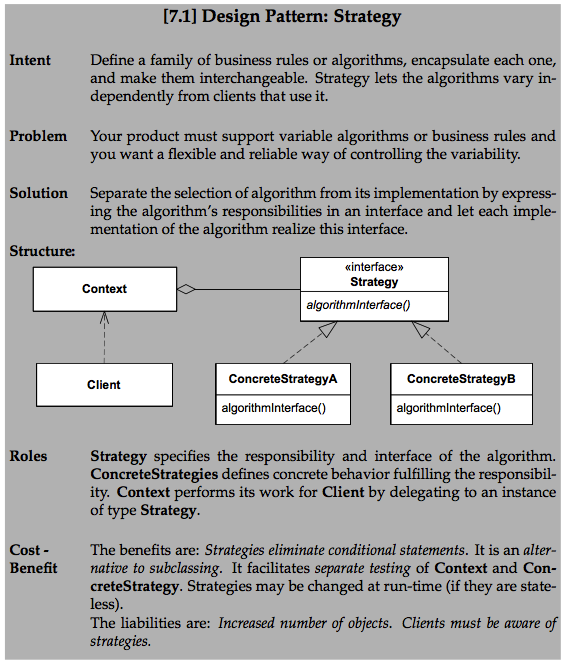
\includegraphics{img/strategy_pattern.png}
\caption{strategy\_pattern.png}
\end{figure}

\hypertarget{state-pattern}{%
\subsection{State Pattern}\label{state-pattern}}

\begin{figure}
\centering
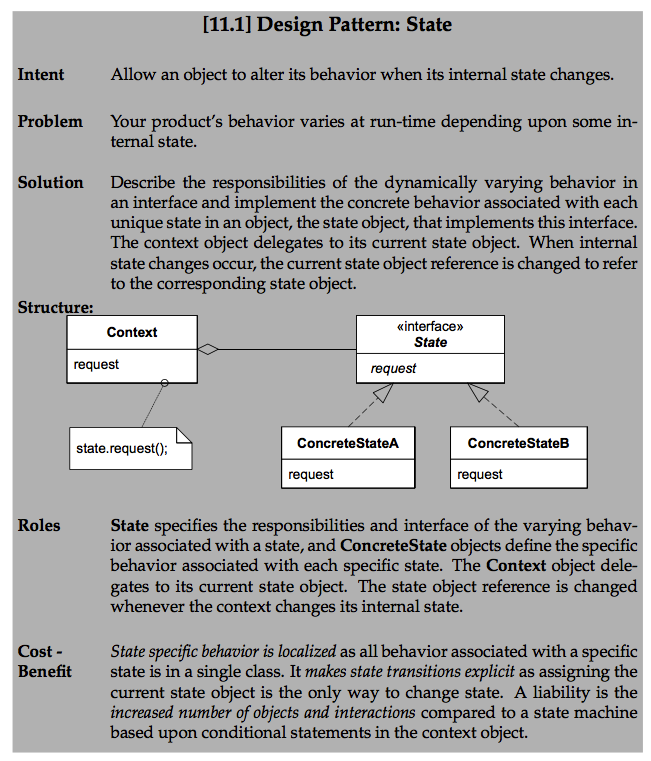
\includegraphics{img/state_pattern.png}
\caption{state\_pattern.png}
\end{figure}

\hypertarget{abstract-factory-pattern}{%
\subsection{Abstract Factory Pattern}\label{abstract-factory-pattern}}

\begin{figure}
\centering
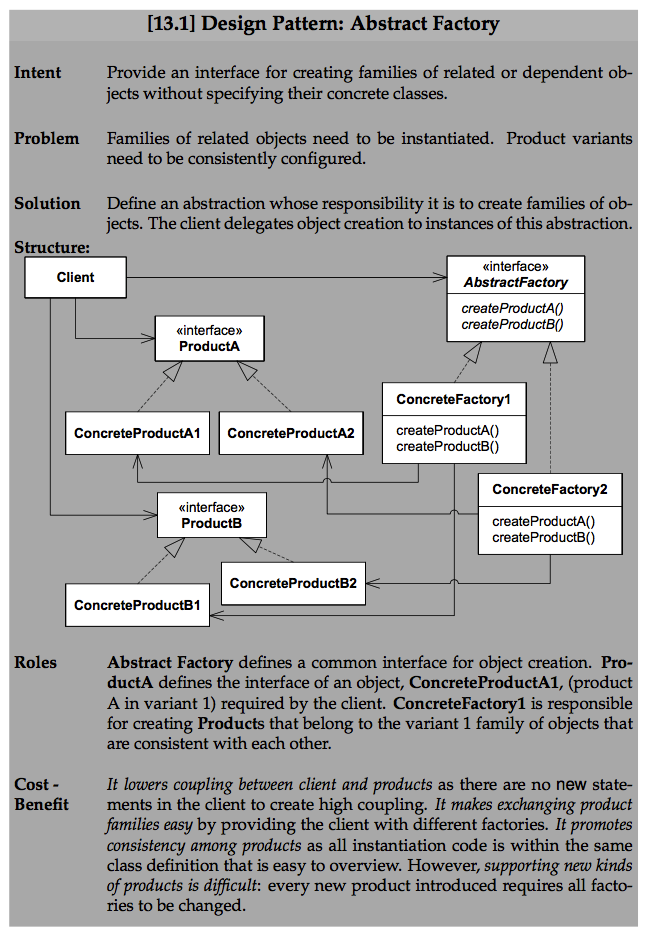
\includegraphics{img/abstract_factory_pattern.png}
\caption{abstract\_factory\_pattern}
\end{figure}

\hypertarget{facade-pattern}{%
\subsection{Facade Pattern}\label{facade-pattern}}

\begin{figure}
\centering
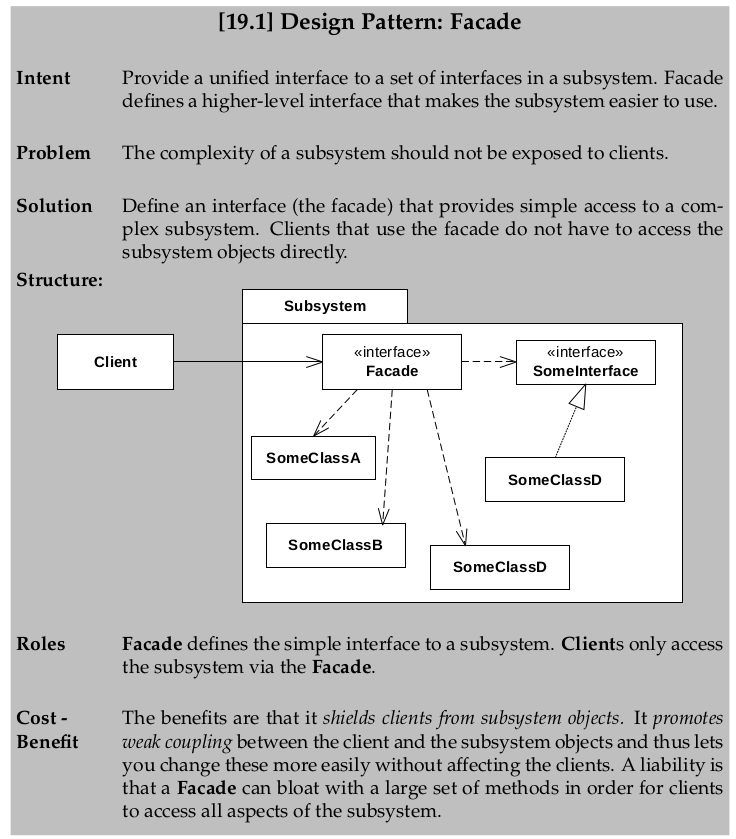
\includegraphics{img/facade_pattern.png}
\caption{facade\_pattern}
\end{figure}

\hypertarget{decorator-pattern}{%
\subsection{Decorator Pattern}\label{decorator-pattern}}

\begin{figure}
\centering
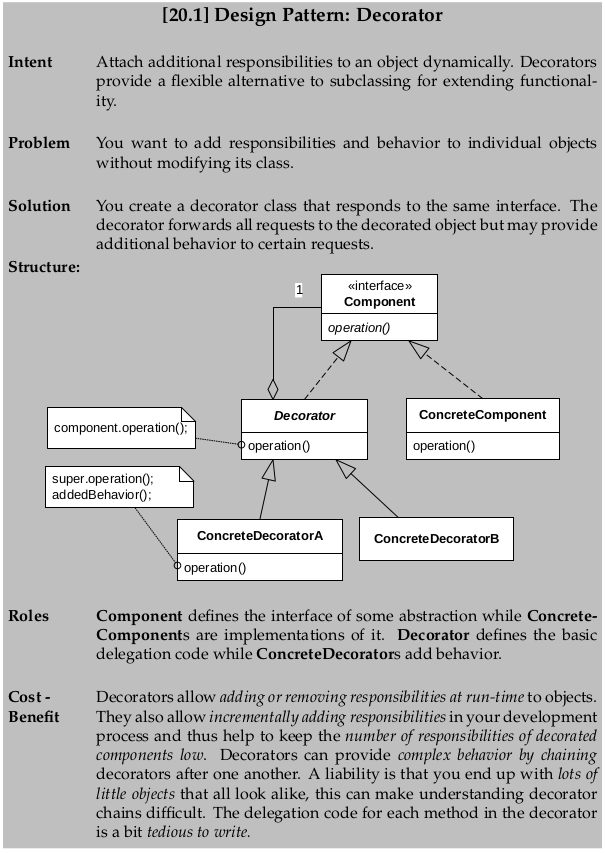
\includegraphics{img/decorator_pattern.png}
\caption{decorator\_pattern}
\end{figure}

\hypertarget{builder-pattern}{%
\subsection{Builder Pattern}\label{builder-pattern}}

\begin{figure}
\centering
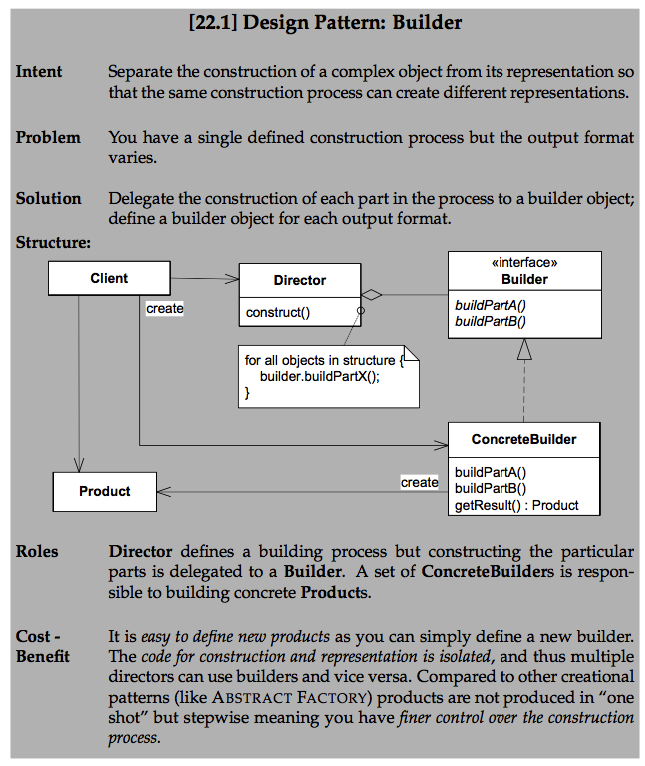
\includegraphics{img/builder_pattern.png}
\caption{builder\_pattern}
\end{figure}

\hypertarget{command-pattern}{%
\subsection{Command Pattern}\label{command-pattern}}

\begin{figure}
\centering
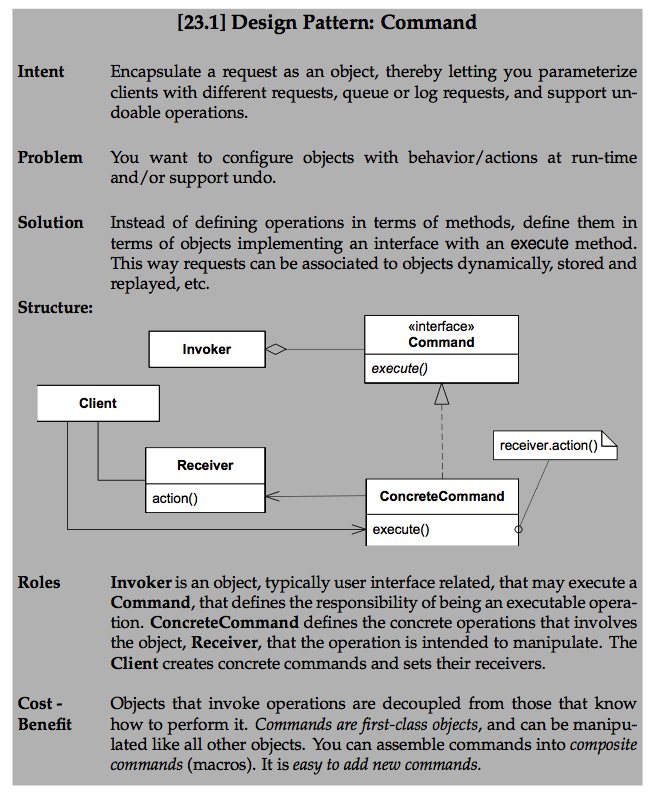
\includegraphics{img/command_pattern.png}
\caption{command\_pattern}
\end{figure}

\hypertarget{proxy-pattern}{%
\subsection{Proxy Pattern}\label{proxy-pattern}}

\begin{figure}
\centering
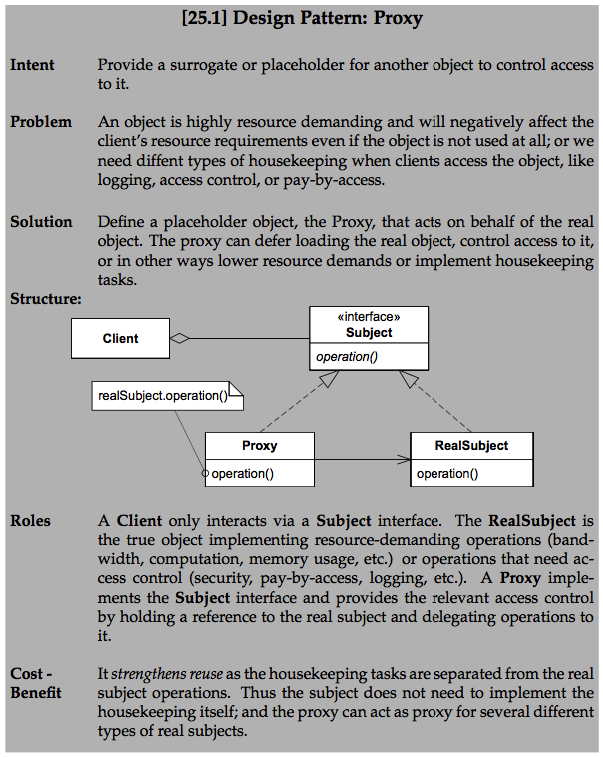
\includegraphics{img/proxy_pattern.png}
\caption{proxy\_pattern}
\end{figure}

\hypertarget{null-object-pattern}{%
\subsection{Null Object Pattern}\label{null-object-pattern}}

\begin{figure}
\centering
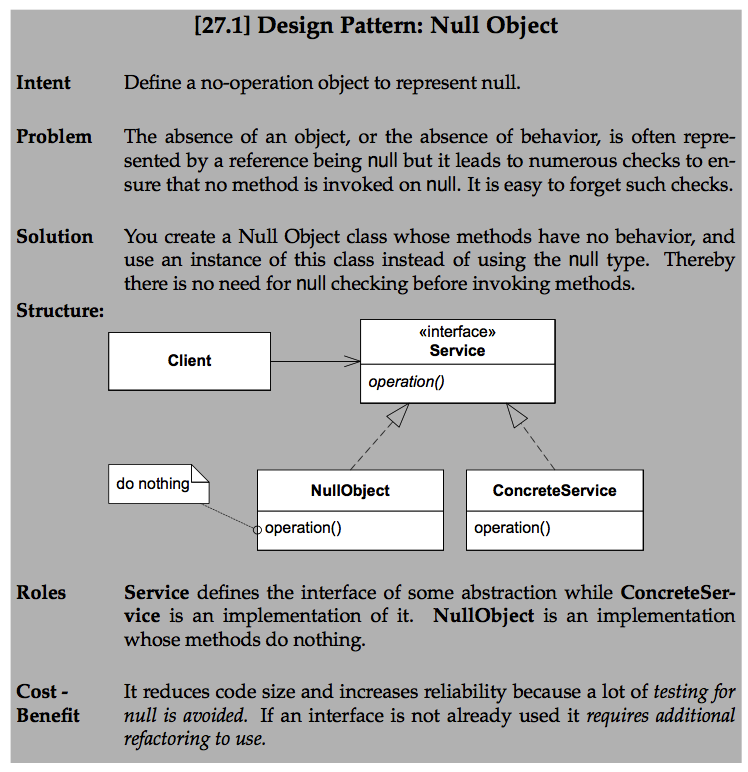
\includegraphics{img/null_object_pattern.png}
\caption{null\_object\_pattern}
\end{figure}

\hypertarget{adapter-pattern}{%
\subsection{Adapter Pattern}\label{adapter-pattern}}

\begin{figure}
\centering
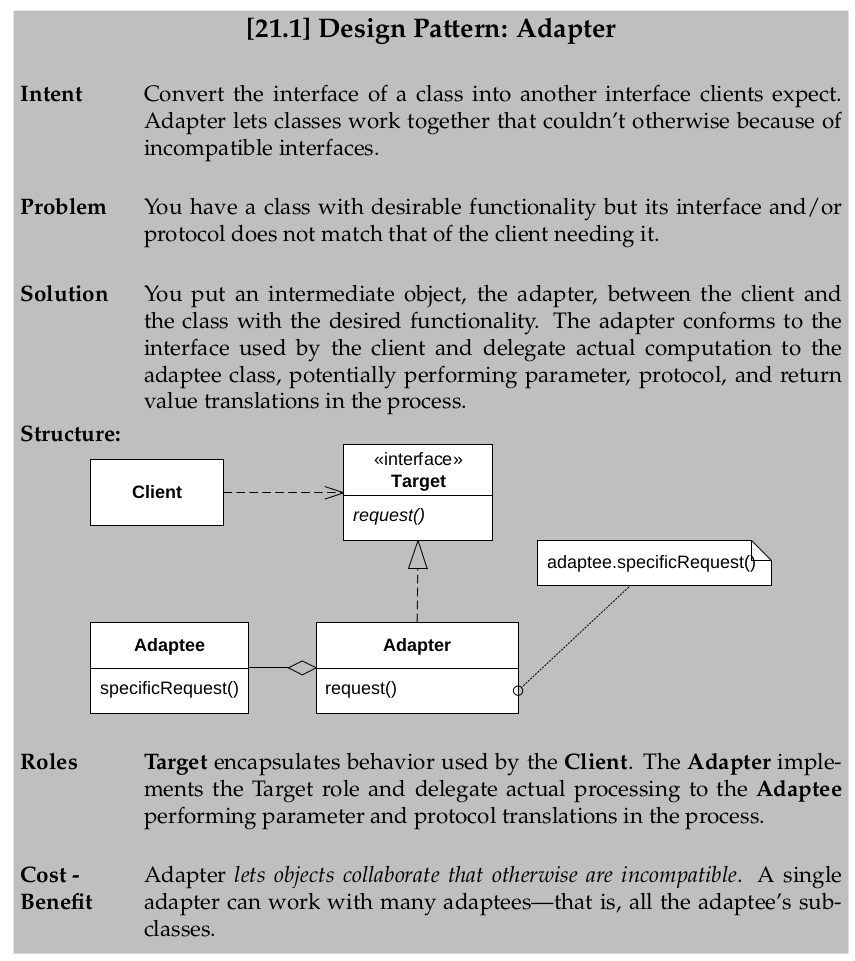
\includegraphics{img/adapter_pattern.png}
\caption{adapter\_pattern}
\end{figure}

\hypertarget{composite-pattern}{%
\subsection{Composite Pattern}\label{composite-pattern}}

\begin{figure}
\centering
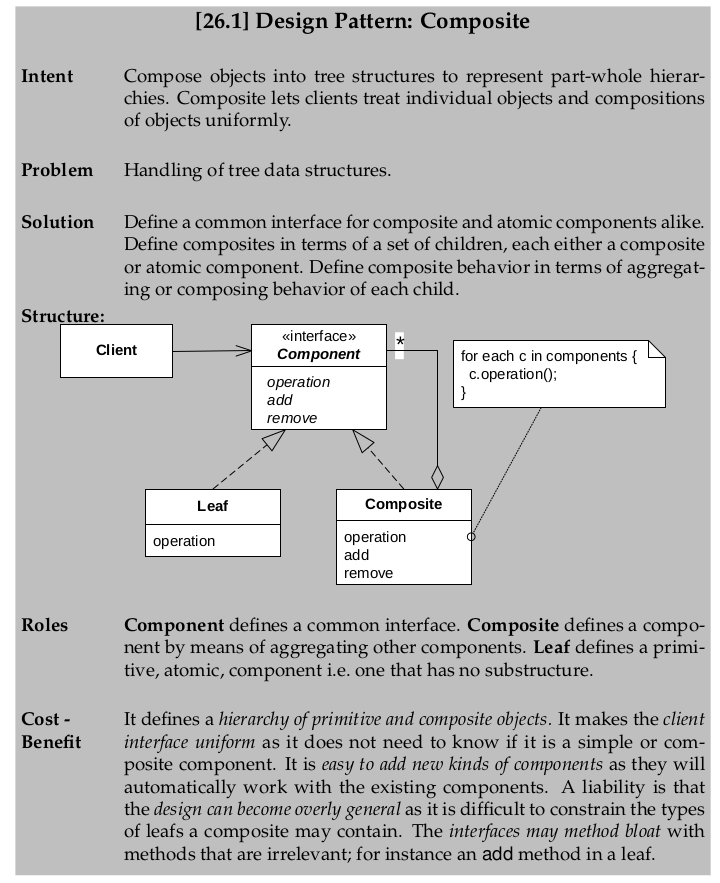
\includegraphics{img/composite_pattern.png}
\caption{composite\_pattern}
\end{figure}

\hypertarget{observer-pattern}{%
\subsection{Observer Pattern}\label{observer-pattern}}

\begin{itemize}
\tightlist
\item
  Push variant: the subject notify the observer with the changed part of
  the state as parameter
\item
  Pull variant: the subject notify the observer that the state has
  changed but not what has changed
\end{itemize}

\begin{figure}
\centering
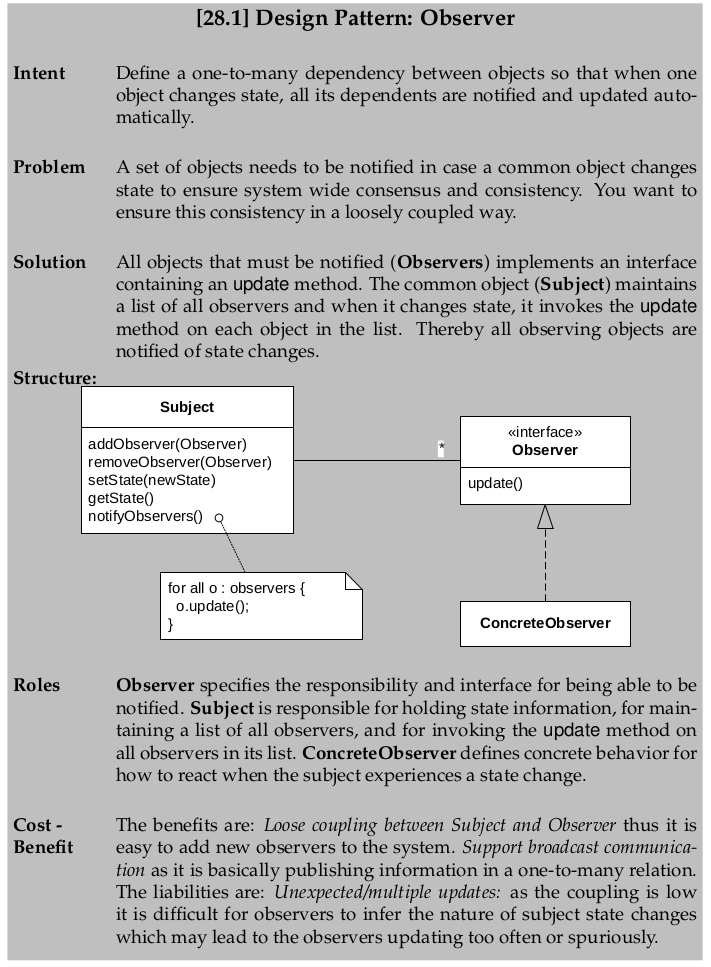
\includegraphics{img/observer_pattern.png}
\caption{observer\_pattern}
\end{figure}

\hypertarget{model-view-controller-pattern}{%
\subsection{Model-View-Controller
Pattern}\label{model-view-controller-pattern}}

\begin{itemize}
\tightlist
\item
  \textbf{Model}

  \begin{itemize}
  \tightlist
  \item
    Store application state
  \item
    Maintain the set of Views associated
  \item
    Notify all view in case of state change
  \end{itemize}
\item
  \textbf{View}

  \begin{itemize}
  \tightlist
  \item
    Visualize model state graphically
  \item
    Accept user input events, delegate them to the associated controller
  \item
    Manage a set of controllers and allow the user to set which
    controller is active
  \end{itemize}
\item
  \textbf{Controller}

  \begin{itemize}
  \tightlist
  \item
    Interpret user input events and translate them into state changes
    for the model
  \end{itemize}
\end{itemize}

\begin{figure}
\centering
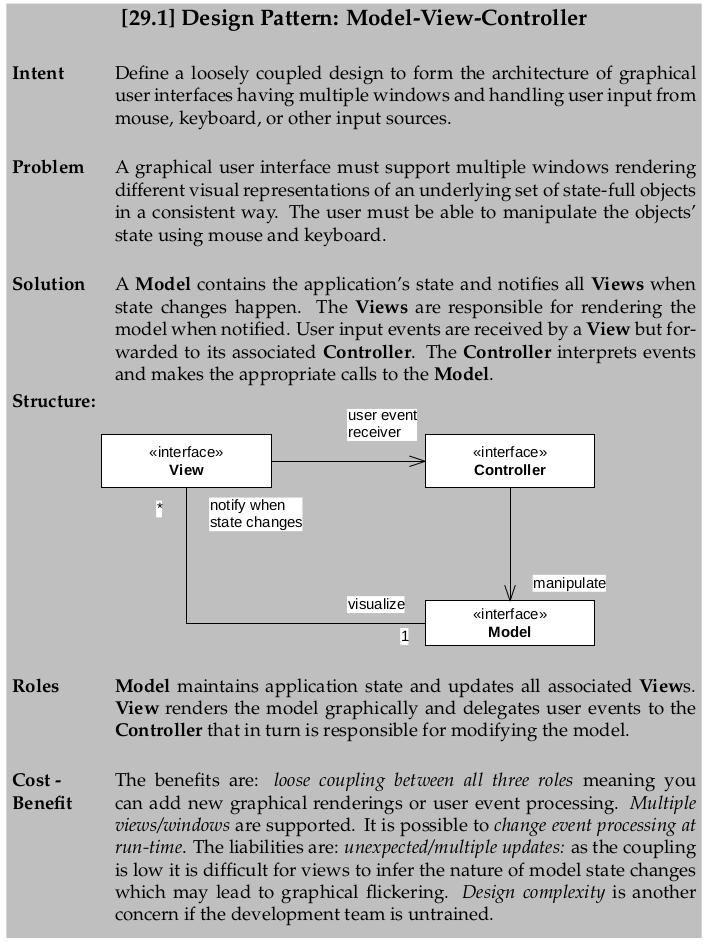
\includegraphics{img/model-view-controller_pattern.png}
\caption{model-view-controller\_pattern}
\end{figure}

\hypertarget{template-method-pattern}{%
\subsection{Template method Pattern}\label{template-method-pattern}}

\begin{itemize}
\tightlist
\item
  \textbf{Unification}

  \begin{itemize}
  \tightlist
  \item
    Both the template method and the hook methods reside in the same
    class
  \item
    The template method is concrete and invokes abstract abstract hook
    methods that can be overridden in a subclass
  \end{itemize}
\item
  \textbf{Separation}

  \begin{itemize}
  \tightlist
  \item
    The template method is defined in one class and the hook methods are
    defined in one or several interfaces
  \item
    The template method is concrete and delegates to implementations of
    the hook interface(s)
    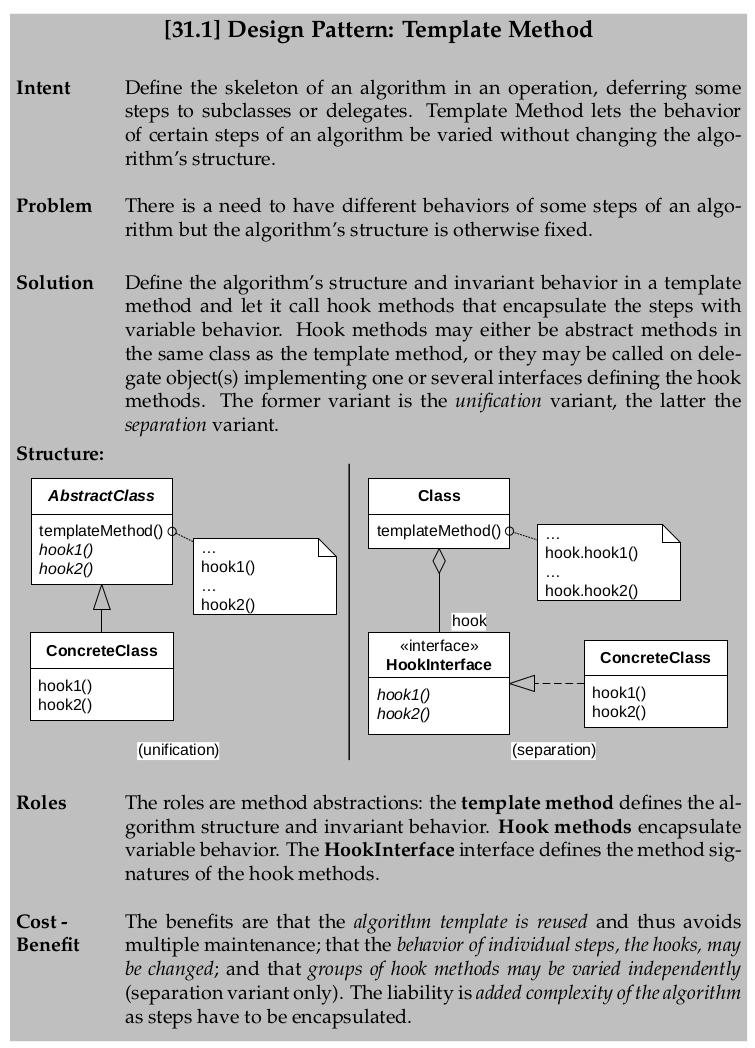
\includegraphics{img/template_method_pattern.png}
  \end{itemize}
\end{itemize}

    \hypertarget{broker-pattern}{%
\subsection{Broker pattern}\label{broker-pattern}}

\begin{itemize}
\tightlist
\item
  \textbf{ClientProxy}

  \begin{itemize}
  \tightlist
  \item
    \texttt{PROXY} for the remote servant object, implements the same
    interface as the servant
  \item
    Translate every method invocations into invocation of the associated
    \textbf{requestor}'s \texttt{request} method
  \end{itemize}
\item
  \textbf{Requestor}

  \begin{itemize}
  \tightlist
  \item
    Perform marshalling of method name and arguments into a
    \textbf{request object}
  \item
    Invoke the \textbf{client request handler}'s \texttt{send} method
  \item
    Demarshal returned \textbf{reply object} into return value(s)
  \item
    Create client side exceptions in case of failures detected at the
    server side
  \end{itemize}
\item
  \textbf{RequestObject}

  \begin{itemize}
  \tightlist
  \item
    Encapsulate all information about a method invocation, including
    object identity, server location, and parameters, in a marshalling
    format.
  \end{itemize}
\item
  \textbf{ClientRequestHandler}

  \begin{itemize}
  \tightlist
  \item
    Perform all \emph{inter process communication} on behalf of the
    client side
  \end{itemize}
\item
  \textbf{ServerRequestHandler}

  \begin{itemize}
  \tightlist
  \item
    Perform all \emph{inter process communication} on behalf of the
    server side
  \item
    Contains the event loop thread that awaits incoming requests from
    the network
  \item
    Upon receiving a message, call the \textbf{Invoker} with the
    received \textbf{RequestObject}
  \end{itemize}
\item
  \textbf{Invoker}

  \begin{itemize}
  \tightlist
  \item
    Perform demarshalling of incoming \textbf{request objects}
  \item
    Determines objects, methods and, arguments and calls the given
    method in the identified \textbf{servant} object
  \item
    Perform marshalling of the return value from the servant object into
    a \textbf{ReplyObject}
  \end{itemize}
\item
  \textbf{ReplyObject}

  \begin{itemize}
  \tightlist
  \item
    Encapsulate all information about return values, including
    exceptions thrown and error descriptions, from a method invocation
    in a marshalling format.
  \end{itemize}
\item
  \textbf{Servant}

  \begin{itemize}
  \tightlist
  \item
    Domain object with the domain implementation on the server side
  \end{itemize}
\item
  Include Format version when using marshalling
\end{itemize}

\begin{figure}
\centering
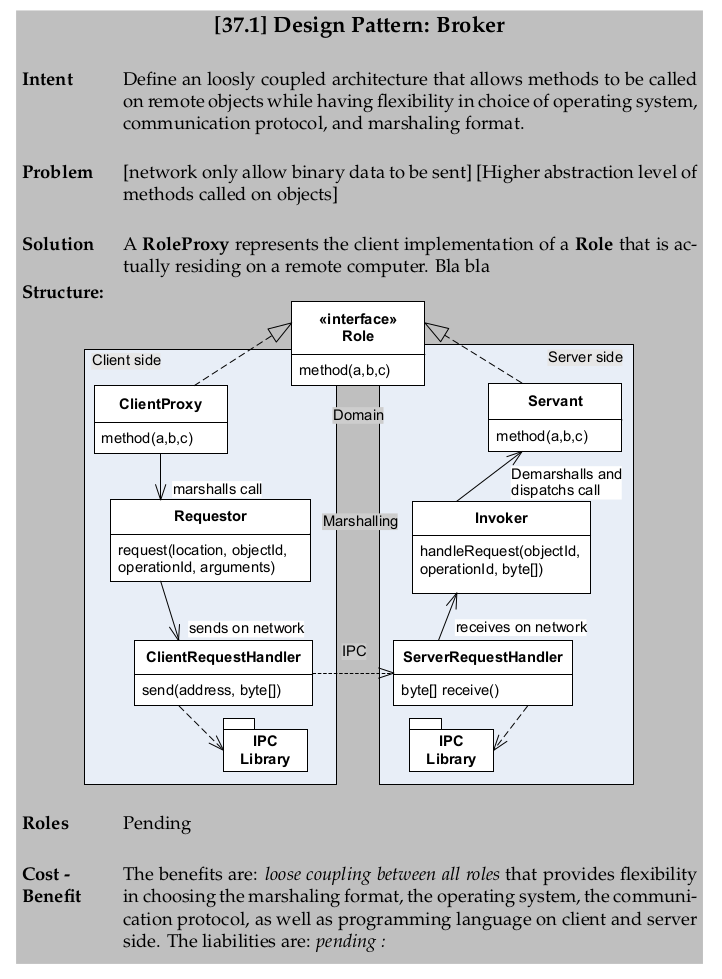
\includegraphics{img/broker_pattern.png}
\caption{broker\_pattern}
\end{figure}

    \hypertarget{clean-code}{%
\section{Clean Code}\label{clean-code}}

\hypertarget{naming}{%
\subsection{Naming}\label{naming}}

\begin{itemize}
\tightlist
\item
  The name of a variable, function or class should reveal it's intention

  \begin{itemize}
  \tightlist
  \item
    Change a name when you find a better one
  \item
    It should tell you

    \begin{itemize}
    \tightlist
    \item
      why it exists
    \item
      what it does
    \item
      how it is used
    \end{itemize}
  \item
    If a name require a comment it does not revel it's intention
  \item
    Classes can be used to avoid magic constants and make the code
    easier to read
  \end{itemize}
\item
  Better names makes the code easier to read
\item
  Do not you names whose entrenched meaning vary from it's intended
  meaning such as \texttt{hp}
\item
  Don't refeer to a grouping of accounts as \texttt{accountList} unless
  it really is a list

  \begin{itemize}
  \tightlist
  \item
    \texttt{accountGroup} or \texttt{accounts} is better
  \end{itemize}
\item
  Do not use name that vary in small ways
\item
  If names must be different they should also mean something different

  \begin{itemize}
  \tightlist
  \item
    Do not use noise word such as \texttt{a} or \texttt{the} to
    differentiate between names
  \item
    Distuinguish names in such a way that the reader knows what the
    differences offer
  \end{itemize}
\item
  The names should be pronousable

  \begin{itemize}
  \tightlist
  \item
    Programming is a social activity
  \end{itemize}
\item
  Use searchable names

  \begin{itemize}
  \tightlist
  \item
    Single letter names or numberic constants are not easy to locate in
    a body of text
  \end{itemize}
\item
  The length of the name should correspond to the size of its scope

  \begin{itemize}
  \tightlist
  \item
    Single letter names can should only be used as local variables
    inside small methods
  \end{itemize}
\item
  Do not use encoded names because they are seldom pronouceable and are
  easy to mistype
\item
  Do not use member prefixes

  \begin{itemize}
  \tightlist
  \item
    Use an IDE that highlights all the important parts of the code
  \end{itemize}
\item
  If you must encode the interface or the implementation chose the
  implementation

  \begin{itemize}
  \tightlist
  \item
    E.g. \texttt{CakeFactory} and \texttt{CakeFactoryImpl}
  \end{itemize}
\item
  Class names should be noun phrase name like \texttt{Customer} or
  \texttt{WikiPage}

  \begin{itemize}
  \tightlist
  \item
    Avoid words like \texttt{Manager}, \texttt{Processor} or
    \texttt{Info} in the name
  \end{itemize}
\item
  Method names should be verbs or verb phrases

  \begin{itemize}
  \tightlist
  \item
    Use the standard prefix in mutator, accesor and predicates:
    \texttt{set}, \texttt{get} and \texttt{is}
  \item
    When constructors are overloaded use static factory methods with
    descriptive names to descripe the arguments

    \begin{itemize}
    \tightlist
    \item
      Enforce this using private constructors
    \end{itemize}
  \end{itemize}
\item
  Do not use ``cute'' name which are jokes.
\item
  Only use one word per concept

  \begin{itemize}
  \tightlist
  \item
    Be sure that the methods with the same name in the different code
    bases does the same
  \end{itemize}
\item
  Use programmer terms to describe methods

  \begin{itemize}
  \tightlist
  \item
    When e.g.~implementing a specific algorithm or pattern
  \end{itemize}
\item
  Add a meaningfull context

  \begin{itemize}
  \tightlist
  \item
    If many variables are part of the same concept prefixes can be
    needed to understand the concepts\\
  \item
    Classes can also be used
  \end{itemize}
\item
  Do not add more to the name as long as they are clear
\end{itemize}

\hypertarget{functions}{%
\subsection{Functions}\label{functions}}

\begin{itemize}
\tightlist
\item
  Function should be small

  \begin{itemize}
  \tightlist
  \item
    The indent level of a function should be no larger than one or two
  \end{itemize}
\item
  Functions should only do one thing

  \begin{itemize}
  \tightlist
  \item
    A way of knowing if a function does more than one thing is that if
    abstracting the code you get a function that is not just a renaming
    of the original function
  \item
    Functions that does more than one thing cannot easily be divided
    into smaller sections
  \end{itemize}
\item
  A function should use the same level of abstraction
\item
  \textbf{The stepdown rule} says that we should be able to read the
  code from top to bottom
\item
  \texttt{Switch} statements should appear once and should be used to
  create polymorfic instances
\item
  Have no side effects of a function

  \begin{itemize}
  \tightlist
  \item
    A function should not do one thing and then another thing hidden
  \item
    The functions should not have a temperal coupling where it is not
    safe to always call a function
  \end{itemize}
\item
  Function should either do something or answer to something not both
\item
  Prefer exception over returning error codes
\item
  Extract the \texttt{try}/\texttt{catch} into their own function

  \begin{itemize}
  \tightlist
  \item
    If the \texttt{try} keyword exists in the function it should be the
    first word and there should be nothing after the catch/finally
    block\\
  \end{itemize}
\item
  \textbf{D}on't \textbf{R}epeat \textbf{Y}ourself
\end{itemize}

\hypertarget{arguments}{%
\subsubsection{Arguments}\label{arguments}}

\begin{itemize}
\tightlist
\item
  The smallest amount of arguments is desireable

  \begin{itemize}
  \tightlist
  \item
    More than three arguments should not be used
  \end{itemize}
\item
  When using a monadic function as an event it should be clear that it
  is an event\\
\item
  If the function is going to transform its input value it should appear
  as an output value
\item
  Flag arguments should be avoided

  \begin{itemize}
  \tightlist
  \item
    It makes the function do more than one thing
  \end{itemize}
\item
  Dyalic functions should avoid when possible

  \begin{itemize}
  \tightlist
  \item
    Harder to read that modadic functions
  \end{itemize}
\item
  Dyalic function should only be used when there is a natural ordering
\item
  When creating function with two or more variable some of the arguments
  can often be wrappen in its own class
\end{itemize}

    \hypertarget{flexibility-and-maintainability}{%
\section{Flexibility and
Maintainability}\label{flexibility-and-maintainability}}

\includegraphics{attachment:maintain.png}\\
- \textbf{Maintainability} (ISO 9126) is the capability of the software
to be modified - Modifications may include correction, improvements,
adaptation to changes, requirements and functional specifications - Can
be messured in how low the cost is to change the software

\begin{itemize}
\item
  \textbf{Analysability} (ISO 9126) is the capability of the software
  product to be diagnosed for deficiencies or cause of failures

  \begin{itemize}
  \tightlist
  \item
    The ability to understand the software
  \item
    It if important to be able to understand and read the software
  \end{itemize}
\item
  \textbf{Changeability} (ISO 9126) is the capability of the software to
  enable specific modification

  \begin{itemize}
  \tightlist
  \item
    The ability to add, modify and enhance a feature in a system as a
    reasonable cost
  \item
    Comes in two flavors

    \begin{itemize}
    \tightlist
    \item
      Those aspects of the software that can be changed at compile time
    \item
      The ones that can be changed at runtime
    \end{itemize}
  \end{itemize}
\item
  \textbf{Stability} (ISO 9126) is the capability of the software to
  avoid unexpected effects from modifications of the system
\item
  \textbf{Testability} (ISO 9126) is the capability of the software to
  enable a modified system to be validated

  \begin{itemize}
  \tightlist
  \item
    The ability to test the software
  \end{itemize}
\item
  \textbf{Flexibility} (ISO 9126) is the capability of the software
  product to support added/enhanced functionality purely by adding
  software units

  \begin{itemize}
  \tightlist
  \item
    The ability to add functionality by adding units
  \item
    Is a special case of changeability
  \end{itemize}
\end{itemize}

    \hypertarget{coupling-and-cohesion}{%
\section{Coupling and Cohesion}\label{coupling-and-cohesion}}

\begin{itemize}
\tightlist
\item
  \textbf{Coupling} is a messure on how strongly depended one software
  unit is on other software units

  \begin{itemize}
  \tightlist
  \item
    Dependencies between software come in many forms

    \begin{itemize}
    \tightlist
    \item
      Methods are depended on the class instance variables
    \item
      Classes are depended on each other when are referenced in code
    \item
      Between packages
    \end{itemize}
  \item
    Tools are available to find couplings
  \item
    Package have light or high coupling
  \item
    High or tight coupling lowers maintainability

    \begin{itemize}
    \tightlist
    \item
      It also lower reliability, because a bug is more likely
    \item
      Becomes harder to read
    \item
      It harder to reuse
    \end{itemize}
  \item
    Week coupling generally make code more relaiable

    \begin{itemize}
    \tightlist
    \item
      It makes code more reliable
    \item
      It is easier to reuse
    \end{itemize}
  \end{itemize}
\item
  \textbf{Cohesion} is a messure on how strongly related and focused the
  responsibilities and provided behaviors of a software unit are.

  \begin{itemize}
  \tightlist
  \item
    Means being organized
  \item
    Is a quality to strive for at all granularities
  \item
    High cohesion means that software units should have few closely
    releated responsability

    \begin{itemize}
    \tightlist
    \item
      Contributes toward reliability and maintainability.
    \item
      Increases the analyzability
    \item
      Make it easier to avoid bugs
    \end{itemize}
  \end{itemize}
\item
  \textbf{Law of Demeter} is do not collaborate with indirect objects

  \begin{itemize}
  \tightlist
  \item
    Also called \emph{``do not talk to stranges''}
  \item
    In a methods you should only invoke methods on

    \begin{itemize}
    \tightlist
    \item
      this
    \item
      a parameter of the method
    \item
      an attribute of this
    \item
      an element in a collection which is an attribute of this
    \item
      an object created within this method
    \end{itemize}
  \item
    Is a design rule rather than law
  \item
    Helps remove high coupling
  \end{itemize}
\end{itemize}

    \hypertarget{test-stubs}{%
\section{Test Stubs}\label{test-stubs}}

\begin{itemize}
\tightlist
\item
  \textbf{Direct input:} is the values or data provided by the test code
  directly that affect the behavior of the unit under test (UUT)
\item
  \textbf{Indirect input:} is the values or data, that can not be
  provided directly by the test code, that affect the behavior of the
  unit under test (UUT)
\item
  \textbf{Depended-on unit (DOU):} A unit in the production code that
  provides values or behavior that affect the behavior of the unit under
  test.
\item
  \textbf{Test stub:} A test stub is a replacement of the real
  depended-on unit that feeds indirect input, defined by the test code,
  into the unit under test \_\_\_
\item
  \textbf{Test stubs make software testable:} Test stubs replace the
  real units and allow the testing code to control the indirect input.
\end{itemize}

    \hypertarget{roles-and-responsibilities}{%
\section{Roles and Responsibilities}\label{roles-and-responsibilities}}

\begin{itemize}
\tightlist
\item
  \textbf{Object-orientation (Model)} A program execution is regarded as
  a physical model simulating the behavior of either a real or imaginary
  part of the world
\item
  \textbf{Object-orientation (Responsibility)} A program is structured
  as a community of interacting agents called object where each object
  has a role to play and performs a service or action used by other
  members
\item
  \textbf{Behavior} acting in a particular and observable way
\item
  \textbf{Responsibility} The state of being accountable and dependable
  to answer a request

  \begin{itemize}
  \tightlist
  \item
    A responsibilities should not be stated too programming specific
    like have an \texttt{addPayment} method
  \item
    Should not be too broad and vague like \emph{``behave like a
    paystation''}
  \end{itemize}
\item
  \textbf{Role (General)} A function or part performed especially in a
  particular operation or process
\item
  The relation between role and object is a many-to-many relation

  \begin{itemize}
  \tightlist
  \item
    A role can be played by many different types of objects
  \item
    A object can perform many different roles within a system
  \end{itemize}
\item
  \textbf{Protocol} A convention detailing the sequence of interaction
  or actions expected by a set of roles\\
\item
  \textbf{Role (Software)} A set of responsibilities and associated
  protocols
\item
  Define small and cohesive roles

  \begin{itemize}
  \tightlist
  \item
    Complex roles may be defined in terms of simpler roles
  \end{itemize}
\end{itemize}

    \hypertarget{systematic-testing}{%
\section{Systematic testing}\label{systematic-testing}}

\begin{itemize}
\tightlist
\item
  \textbf{Systematic testing} is a planned and systematic process with
  an explicit goal of finding defects in some well-defined part of the
  system

  \begin{itemize}
  \tightlist
  \item
    The criteria of success is to prove that the system does no work
  \end{itemize}
\item
  \textbf{Black-box testing}: the unit under test (UUT) is treated like
  a black box

  \begin{itemize}
  \tightlist
  \item
    The only knowledge we have to guide the testing is the specification
    of the UUT and general programming techniques, algorithmic
    constructs and common mistakes made by programmers
  \end{itemize}
\item
  \textbf{White-box testing}: The full implementation of the code is
  known so the actual code can be inspected to make test cases
\item
  The following testing approaches should be used based on the
  complexity of the UUT

  \begin{itemize}
  \tightlist
  \item
    \textbf{No testing} Many methods are so small that they are not
    worth testing

    \begin{itemize}
    \tightlist
    \item
      Examples are the accessor methods
    \end{itemize}
  \item
    \textbf{Explorative test} are test based on experience and gut
    feeling but you do not follow any rigid method

    \begin{itemize}
    \tightlist
    \item
      are well suited for medium complex methods
    \item
      are characterized by their low cost
    \item
      is used in TDD
    \end{itemize}
  \item
    \textbf{Systematic testing} is were you follow a rigid method for
    generating test cases

    \begin{itemize}
    \tightlist
    \item
      is costly as quite a lot of effort is invested in careful analysis
      of the problem
    \item
      is best suited for highly complex methods were the time invested
      are worthwhile
    \end{itemize}
  \end{itemize}
\end{itemize}

\hypertarget{equivalence-class-partitioning}{%
\subsection{Equivalence class
partitioning}\label{equivalence-class-partitioning}}

\begin{itemize}
\item
  The process of equivalence partitioning is roughly the same every time

  \begin{enumerate}
  \def\labelenumi{\arabic{enumi}.}
  \tightlist
  \item
    Review the requirements for the UUT and identify conditions and use
    heuristics to find ECs for each condition
  \item
    Review the produced ECs and consider carefully the representation
    property of elements in each EC

    \begin{itemize}
    \tightlist
    \item
      If you question if a particular elements is representative for the
      EC then repartition the EC
    \item
      Best documented using a EC table
    \end{itemize}
  \item
    Review to verify that the coverage property is fulfilled
  \item
    Generate test cases from the ECs

    \begin{itemize}
    \tightlist
    \item
      Use Myers heuristics for combination to generate a minimal set of
      test cases\\
    \item
      Best documented using a test case table \_\_\_
    \end{itemize}
  \end{enumerate}
\item
  \textbf{Equivalence class} a subset of all possible values to the UUT
  that has the property that if one element in the subset demonstrates a
  defect during testing, then we can assume that all other elements in
  that subset will produce the same defect
\item
  When partitioning the input space into EC two properties must be
  fulfilled in order for the partitioning to be sound

  \begin{itemize}
  \tightlist
  \item
    \textbf{Coverage:} Every possible input element belongs to at least
    one of the equivalence classes
  \item
    \textbf{Representation:} If a defect is demonstrated on a particular
    member of an equivalence class, the same defect is assumed to be
    demonstrated by any other member of the class.
  \end{itemize}
\item
  An invalid EC is defined as values that makes the method bail out
  early in the algorithm by using simple switches
\item
  To document a set of ECs a \textbf{equivalence class table} is often
  used

  \begin{itemize}
  \tightlist
  \item
    e.g.~for the \texttt{Math.abs} function in java
    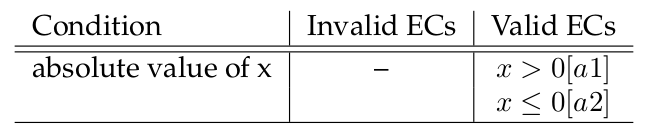
\includegraphics{img/equivalence_table.png} \_\_\_
  \end{itemize}
\item
  A good source for partitioning is to look for \textbf{conditions} in
  the specification of the UUT

  \begin{itemize}
  \tightlist
  \item
    is often associated with input values
  \item
    is also sometimes associated with the output values
  \end{itemize}
\item
  Given a condition, you can derive the first set of ECs following the
  guidelines:

  \begin{itemize}
  \tightlist
  \item
    \textbf{Range:} If a condition is specified for a range of values

    \begin{itemize}
    \tightlist
    \item
      Select one valid EC that covers the allowed range and two invalid
      one above and one below
    \end{itemize}
  \item
    \textbf{Set:} If a condition is specified for a set of values

    \begin{itemize}
    \tightlist
    \item
      Define a EC for each value in the set and one for all the values
      outside the set
    \end{itemize}
  \item
    \textbf{Boolean:} If a condition is specified as a must-be condition

    \begin{itemize}
    \tightlist
    \item
      Define one EC for the condition being true and one EC for it being
      false \_\_\_
    \end{itemize}
  \end{itemize}
\item
  If the specification of the UUT test defines an arithmetic operation
  then

  \begin{itemize}
  \tightlist
  \item
    \textbf{Addition and subtraction} If a computation includes addition
    or subtraction

    \begin{itemize}
    \tightlist
    \item
      Select one valid EC for the natural element 0 and one valid EC for
      all other elements
    \end{itemize}
  \item
    \textbf{Multiplication and division} If a computation includes
    multiplication or division

    \begin{itemize}
    \tightlist
    \item
      Select one valid EC for the natural element 1 and one valid EC for
      all other elements
    \end{itemize}
  \end{itemize}
\item
  The heuristic for a arithmetic operation must be applied to all
  elements in the computation \_\_\_
\item
  To limit the number of test cases the \textbf{Myers heuristics} can be
  used:

  \begin{enumerate}
  \def\labelenumi{\arabic{enumi}.}
  \tightlist
  \item
    Until all valid EC has been covered define a test case that covers
    as many uncovered valid ECs as possible
  \item
    Until all invalid ECs have been covered, define a test case whose
    element only lies in a single invalid ECs.
  \end{enumerate}
\item
  For computations define test cases that only include ECs with
  non-neutral elements\\
\item
  Example of a test-case table 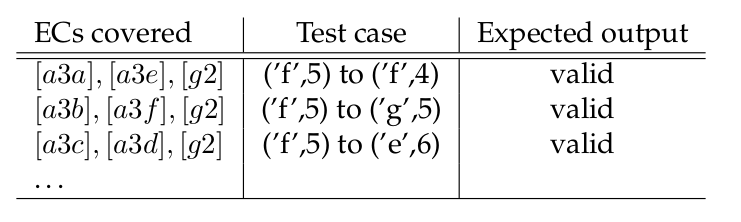
\includegraphics{img/test_case_table.png}
  \_\_\_
\item
  A \textbf{boundary value} is a value that lies right on the edge of an
  equivalence class
\item
  \textbf{Observe unit preconditions}

  \begin{itemize}
  \tightlist
  \item
    Do not generate test cases for conditions that a unit specifically
    cannot or should not handle.
  \end{itemize}
\item
  \textbf{Systematic testing assumes competent programmers}

  \begin{itemize}
  \tightlist
  \item
    Equivalence partitioning and other testing techniques rely on honest
    and competent programmers that are using standard techniques.
  \end{itemize}
\item
  \textbf{Do not use Myers combination heuristics blindly}

  \begin{itemize}
  \tightlist
  \item
    Myers heuristics for generating test cases from valid and invalid
    ECs can lead to omitting important test cases.
  \end{itemize}
\end{itemize}

    \hypertarget{framework-theory}{%
\section{Framework Theory}\label{framework-theory}}

\begin{itemize}
\tightlist
\item
  Framework characteristics are

  \begin{itemize}
  \tightlist
  \item
    Skeleton / design / high-level language / template

    \begin{itemize}
    \tightlist
    \item
      a framework delivers application behavior at a high level of
      abstraction
    \end{itemize}
  \item
    Application / class of software / within a domain

    \begin{itemize}
    \tightlist
    \item
      a framework provides behavior in a well defined domain
    \end{itemize}
  \item
    Cooperating / collaborating classes

    \begin{itemize}
    \tightlist
    \item
      a framework defines the protocol between a set of well-defined
      components / objects
    \item
      to use a framework you have to understand the protocol
    \end{itemize}
  \item
    Customize / abstract classes / reusable / specialize

    \begin{itemize}
    \tightlist
    \item
      the framework is flexible, so you can tailor it to a concrete
      context, as long as the context lies within the domain of the
      framework
    \end{itemize}
  \item
    Classes / implementation / skeleton

    \begin{itemize}
    \tightlist
    \item
      a framework is reuse of working code as well as reuse of design
    \end{itemize}
  \end{itemize}
\item
  Inversion of control

  \begin{itemize}
  \tightlist
  \item
    The frameworks defines the flow of control not you
  \item
    Often described using the Hollywood principle \emph{``Don't call us
    we'll call you''}
  \item
    example of framework vs library
    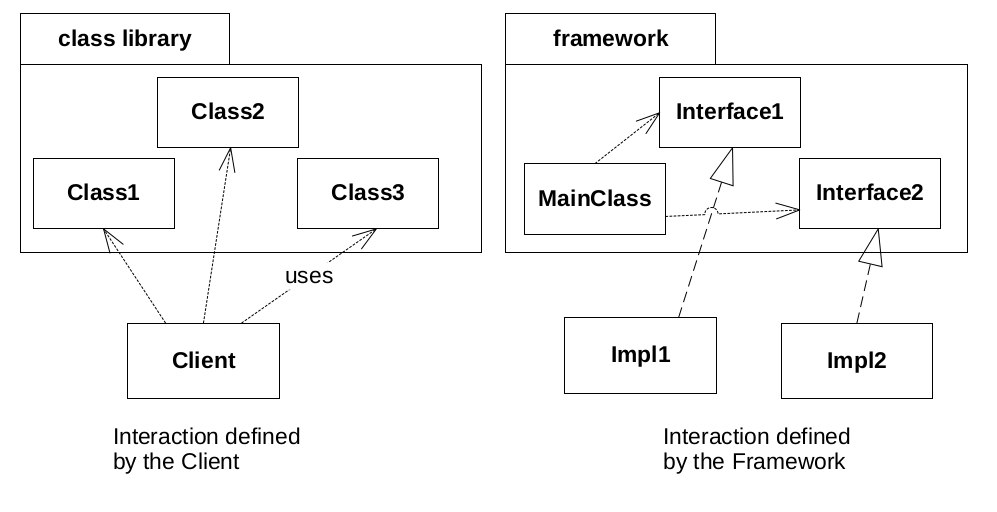
\includegraphics{img/inversion_of_control.png}
  \end{itemize}
\item
  Framework reuse is reuse of both design and code

  \begin{itemize}
  \tightlist
  \item
    A framework is a tangible unit of software, thus it is code reuse
  \item
    Due to the inversion on control property it also defines

    \begin{itemize}
    \tightlist
    \item
      flow of control
    \item
      object protocols
    \item
      variability point
    \end{itemize}
  \item
    Also bundles a quality design
  \end{itemize}
\item
  \textbf{Software product line}: A software product line is a set of
  software intensive systems sharing a common, managed set of features
  that satisfy the specific needs of a particular market segment or
  mission and that are developed from a common set of core assets in a
  prescribed way.
\end{itemize}

\hypertarget{types-of-users-and-developers}{%
\subsection{Types of users and
developers}\label{types-of-users-and-developers}}

\begin{itemize}
\tightlist
\item
  When doing framework development there are three types of stakeholders

  \begin{enumerate}
  \def\labelenumi{\arabic{enumi}.}
  \tightlist
  \item
    Framework developers

    \begin{itemize}
    \tightlist
    \item
      The people that design and program the framework
    \end{itemize}
  \item
    Application developers

    \begin{itemize}
    \tightlist
    \item
      are the developers that uses the framework in order to make an
      applications
    \item
      the users of the framework
    \end{itemize}
  \item
    Users
  \end{enumerate}
\item
  Things to consider when developering a framework in respect to the
  application developers are

  \begin{itemize}
  \tightlist
  \item
    the frameworks domain must be sufficiently close to the domain that
    the application developers are trying to address
  \item
    the framework must be flexible so the application developer can
    adopt it for a specific context
  \item
    the framework must deliver design, functionality and domain
    knowledge that otherwise is very expensive to acquire

    \begin{itemize}
    \tightlist
    \item
      This speaks in favor of frameworks of some complexity and size
    \end{itemize}
  \item
    the framework must be reliable
  \end{itemize}
\item
  Successful use relies on that the application developers

  \begin{itemize}
  \tightlist
  \item
    understand the protocols between the framework and the customization
    code they provide
  \item
    understand the aspects that can (and cannot) be customized as well
    as the concrete techniques used for the customization
  \end{itemize}
\end{itemize}

\hypertarget{frozen-and-hot-spots}{%
\subsection{Frozen and Hot Spots}\label{frozen-and-hot-spots}}

\begin{itemize}
\tightlist
\item
  \textbf{Frozen spot}

  \begin{itemize}
  \tightlist
  \item
    a part of framework code that cannot be altered
  \item
    defines the basic design and the object protocols in the final
    application
  \end{itemize}
\item
  \textbf{Hot spot}

  \begin{itemize}
  \tightlist
  \item
    a clearly defined part of the framework
  \item
    specialization code can alter or add behavior to the application
    \_\_\_
  \end{itemize}
\item
  Frameworks are not customized by code modification

  \begin{itemize}
  \tightlist
  \item
    A framework is a closed black box in which the source code must not
    be altered
  \item
    Customization must only take place through providing behavior in the
    hot spots by those mechanisms laid out by the framework developers
  \item
    Change by addition not modification
  \end{itemize}
\item
  Another term for hot spot can be a hook variability points

  \begin{itemize}
  \tightlist
  \item
    Many frameworks come with standard implementation for most or all
    the variability points
  \end{itemize}
\item
  Framework code is code that defines the framework
\item
  Application code is code that defines the specialisation of the
  variability points
\end{itemize}

\hypertarget{defining-variability-points}{%
\subsection{Defining Variability
Points}\label{defining-variability-points}}

\begin{itemize}
\item
  Frameworks must use dependency injection

  \begin{itemize}
  \tightlist
  \item
    frameworks themselves cannot instantiate objects that define
    variability points
  \item
    the variability points themselves have to be instantiated by the
    application code and injected into the framework
  \end{itemize}
\item
  A hands-on rule is that framework code must never contain a new
  statement classes that have hot spot methods defined
\item
  Frameworks present a range of possibilities for defining the hot spot
  objects

  \begin{itemize}
  \tightlist
  \item
    Existing concrete classes

    \begin{itemize}
    \tightlist
    \item
      The framework comes with a number of predefined classes
    \item
      It is your job to compose the predefined classes into something
      sensible
    \item
      Examples include AWT and Swing where you compose new graphical
      user interfaces from predefined components
    \end{itemize}
  \item
    Subclassing and abstract class

    \begin{itemize}
    \tightlist
    \item
      the framework contains abstract classes
    \item
      most of a high quality implementation is already given
    \item
      the developer must fill out the last details
    \end{itemize}
  \item
    Implementing an interface

    \begin{itemize}
    \tightlist
    \item
      the framework contains an interface
    \item
      gives the application developer the opportunity to exercise full
      control over the hot spots.
    \end{itemize}
  \end{itemize}
\item
  A framework should support the spectrum from no implementation
  (interface) over partial (abstract) to full (concrete) implementation
  for variability points
\end{itemize}

    \hypertarget{modifiability}{%
\section{Modifiability}\label{modifiability}}

\begin{itemize}
\tightlist
\item
  \textbf{Modifiability} is about change and the interest in it centers
  on costs and risks
\item
  To plan for modifiability the architects has to consider four
  questions

  \begin{enumerate}
  \def\labelenumi{\arabic{enumi}.}
  \tightlist
  \item
    \emph{What can change?}

    \begin{itemize}
    \tightlist
    \item
      the functions the system computes
    \item
      the platform
    \item
      the environment
    \item
      the qualities (performance, reliability and even its future
      modification)
    \end{itemize}
  \item
    \emph{What is the likelihood of the change?}

    \begin{itemize}
    \tightlist
    \item
      it is not possible to plan for all potential chagnes
    \item
      the architect must make tough decisions about which changes are
      likely
    \end{itemize}
  \item
    \emph{When is the change made and who makes it?}

    \begin{itemize}
    \tightlist
    \item
      the change is commonly made in the source code
    \item
      a change can be made by a developer, an end user, or a system
      administrator
    \end{itemize}
  \item
    \emph{What is the cost of the change?}

    \begin{itemize}
    \tightlist
    \item
      making a system more modifiable involves two types of cost:

      \begin{itemize}
      \tightlist
      \item
        The cost of introducing the mechanism(s) to make the system more
        modifiable
      \item
        The cost of making the modification using the mechanism(s)
      \end{itemize}
    \end{itemize}
  \end{enumerate}
\item
  To calculate weather a introducing a mechanism to make the system more
  modifiable is worth is the following formular is used. \(N\) is the
  anticipated number of modfication that will use the mechanism, but it
  is an prediction 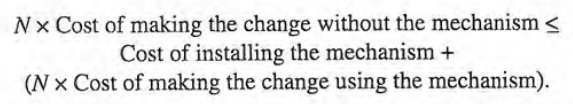
\includegraphics{img/modification_formular.png}
\end{itemize}

    \hypertarget{general-scenario}{%
\subsection{General Scenario}\label{general-scenario}}

\begin{itemize}
\item
  From these consideration, we can see the portions of the modifiability
  general scenario

  \begin{itemize}
  \tightlist
  \item
    \textbf{Source of stimulus}

    \begin{itemize}
    \tightlist
    \item
      specifies who makes the change; the developer; a system
      administrator; or an end user
    \end{itemize}
  \item
    \textbf{Stimulus}

    \begin{itemize}
    \tightlist
    \item
      specifies the change to be made
    \item
      can be

      \begin{itemize}
      \tightlist
      \item
        the addition of a function
      \item
        modification of an existing function
      \item
        deletion of a function
      \end{itemize}
    \item
      can also be made to the qualities of the system

      \begin{itemize}
      \tightlist
      \item
        e.g.~making it more responsive
      \end{itemize}
    \item
      can also be made to the capacity of the system
    \item
      can also be done to accommodate new technology of some sort
    \end{itemize}
  \item
    \textbf{Artifact}

    \begin{itemize}
    \tightlist
    \item
      specifies what is to be changed
    \end{itemize}
  \item
    \textbf{Environment}

    \begin{itemize}
    \tightlist
    \item
      specifies when the change can be made
    \end{itemize}
  \item
    \textbf{Response}

    \begin{itemize}
    \tightlist
    \item
      make the change, test it and deploy it
    \end{itemize}
  \item
    \textbf{Response measure}

    \begin{itemize}
    \tightlist
    \item
      most common measures are time and money of responses
    \end{itemize}
  \end{itemize}
\item
  Example 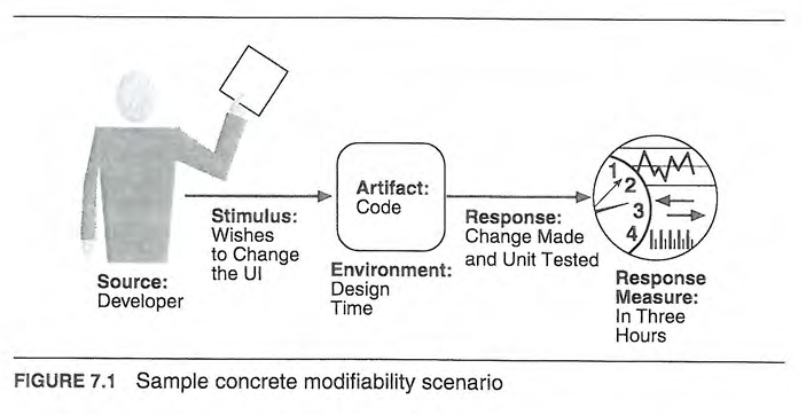
\includegraphics{img/modification_example.png}
\item
  Modifiability General Scenario
  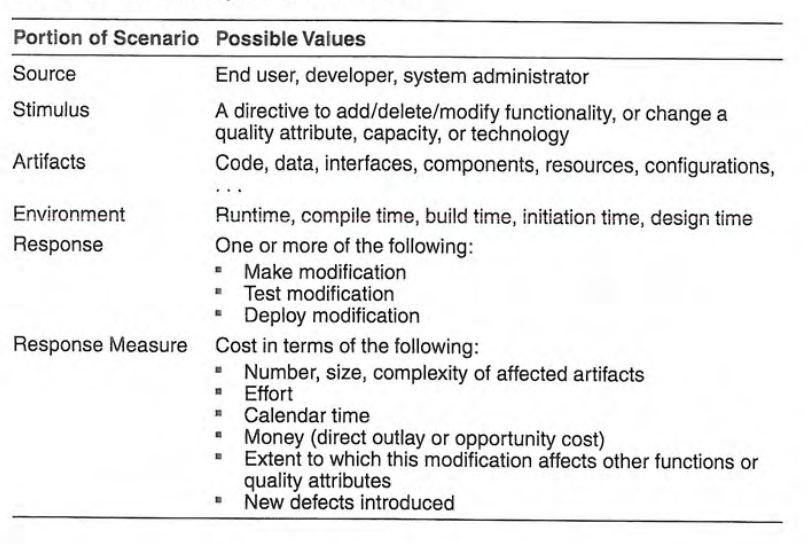
\includegraphics{img/modification_general.png}
\end{itemize}

    \hypertarget{distributed-computing}{%
\section{Distributed computing}\label{distributed-computing}}

\begin{itemize}
\tightlist
\item
  Distributed computing is the field in computer science that studies
  distributed systems
\item
  \textbf{Distributed system} is one in which components located at
  networked computers communicate and coordinate their action only by
  passing messages
\item
  \textbf{Client-sever architecture}

  \begin{itemize}
  \tightlist
  \item
    Two components need to communicate and are independent of each other

    \begin{itemize}
    \tightlist
    \item
      One of the components is indicating a connection for a service
      that the other one provides
    \item
      The component providing a service must be able to cope with
      numerous connections at a time
    \item
      The requesting component must be able deal with different results
    \end{itemize}
  \item
    The CLIENT-SERVER pattern distinguishes two kinds of components
    clients and servers

    \begin{itemize}
    \tightlist
    \item
      The client request information or services from a server which
      means it needs to known

      \begin{itemize}
      \tightlist
      \item
        how to access the server which requires and ID or and address to
        the server
      \item
        the interface of the server
      \end{itemize}
    \item
      The server responds to requests from the client

      \begin{itemize}
      \tightlist
      \item
        processes each request on its own
      \item
        does not know the ID or the address of the client before the
        interactions
      \end{itemize}
    \item
      Clients are optimized for their application task
    \item
      Servers are optimized for serving multiple clients. \_\_\_
    \end{itemize}
  \end{itemize}
\item
  \textbf{Request-Reply protocol} simulate a synchroneous call between
  client and a server objects by pairwise exchange of messages

  \begin{itemize}
  \tightlist
  \item
    one forming the request message from client to server
  \item
    second forming the reply message from server back to client
  \item
    the client sends the request message, and waits/blocks until the
    reply message has been received.
    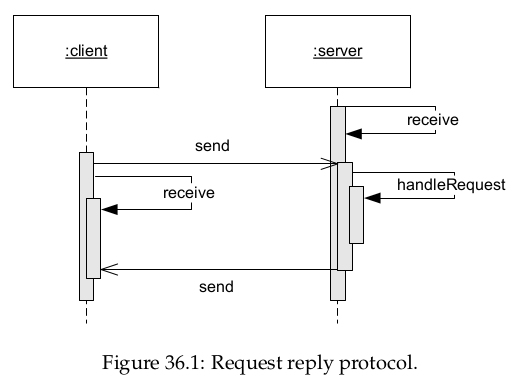
\includegraphics{img/request_reply.png}
  \end{itemize}
\end{itemize}

\begin{center}\rule{0.5\linewidth}{\linethickness}\end{center}

\begin{itemize}
\tightlist
\item
  \textbf{Marshalling} is the process of taking a collection of
  structured data items and assembling them into a byte array suitable
  for transmission in a network message
\item
  \textbf{Unmarshalling} is the process of disassembling a byte array
  received in network message to produce the equivalent collection of
  structured data items.
\item
  The Marshalling and Unmarshalling process has to agree on the format
  used, the marshalling format.

  \begin{itemize}
  \tightlist
  \item
    Google's Gson library can be used for marshalling and unmarshalling
    JSON \_\_\_\_
  \end{itemize}
\item
  \textbf{Named services} can be used to translate from a name of the
  remote object to the actual location and identity of it

  \begin{itemize}
  \tightlist
  \item
    Java RMI provides a registry where you can bind a name with a
    location
  \item
    DNS servers binds url e.g. \texttt{google.dk} to actual ip-address
  \end{itemize}
\end{itemize}

    \hypertarget{concurrency}{%
\section{Concurrency}\label{concurrency}}

\begin{itemize}
\tightlist
\item
  \texttt{java.util.concurrent.locks} contains multiple lock
  implementations
\end{itemize}

\hypertarget{creating-and-starting}{%
\subsection{Creating and starting}\label{creating-and-starting}}

\begin{itemize}
\tightlist
\item
  Creating a thread is done the following way
\end{itemize}

\begin{Shaded}
\begin{Highlighting}[]
\BuiltInTok{Thread}\NormalTok{ thread = }\KeywordTok{new} \BuiltInTok{Thread}\NormalTok{();}
\end{Highlighting}
\end{Shaded}

\begin{itemize}
\tightlist
\item
  To start a thread its \texttt{start} method is called
\end{itemize}

\begin{Shaded}
\begin{Highlighting}[]
\NormalTok{thread.}\FunctionTok{start}\NormalTok{();    }
\end{Highlighting}
\end{Shaded}

\begin{itemize}
\tightlist
\item
  One way to create a thread is to subclass thread and override it's
  \texttt{run} method

  \begin{itemize}
  \tightlist
  \item
    This can also be done anonymously
  \end{itemize}
\item
  Another way to create a thread is to implement the interface
  \texttt{Runnable} and give one to the thread constructor. - Threads
  can be names by given a string as and argument to the constructor

  \begin{itemize}
  \tightlist
  \item
    To get the name of a given thread the \texttt{getName} method is
    used
  \end{itemize}
\item
  To get the current running thread \texttt{Thread.currentThread()} can
  be used
\end{itemize}

    \hypertarget{race-conditions}{%
\subsection{Race conditions}\label{race-conditions}}

\begin{itemize}
\tightlist
\item
  A \textbf{critical section} is a section of the code that is executed
  by multiple threads and where the sequence of execution of threads
  makes a difference in the result of the concurrent execution of the
  critical section
\item
  A \textbf{race condition} is a special condition that might occur
  inside a critical section

  \begin{itemize}
  \tightlist
  \item
    When the result of multiple threads executing a critical section may
    differ depending on the sequence in which the threads execute, the
    critical section is said to contain a race condition.
  \item
    Problems only arise when multiple threads write to the same resource
  \end{itemize}
\item
  To prevent race conditions from happening the critical section must be
  executed as an atomic instruction
\item
  Race conditions can be avoided using proper thread synchronization

  \begin{itemize}
  \tightlist
  \item
    can be achieved using synchronized block of Java code e.g.
  \end{itemize}

\begin{Shaded}
\begin{Highlighting}[]
  \KeywordTok{public} \KeywordTok{class}\NormalTok{ TwoSums \{    }
      \KeywordTok{private} \DataTypeTok{int}\NormalTok{ sum1 = }\DecValTok{0}\NormalTok{;}
      \KeywordTok{private} \DataTypeTok{int}\NormalTok{ sum2 = }\DecValTok{0}\NormalTok{;}

      \KeywordTok{public} \DataTypeTok{void} \FunctionTok{add}\NormalTok{(}\DataTypeTok{int}\NormalTok{ val1, }\DataTypeTok{int}\NormalTok{ val2)\{}
          \KeywordTok{synchronized}\NormalTok{(}\KeywordTok{this}\NormalTok{)\{}
              \KeywordTok{this}\NormalTok{.}\FunctionTok{sum1}\NormalTok{ += val1;   }
              \KeywordTok{this}\NormalTok{.}\FunctionTok{sum2}\NormalTok{ += val2;}
\NormalTok{          \}}
\NormalTok{      \}}
\NormalTok{  \}}
\end{Highlighting}
\end{Shaded}

  \begin{itemize}
  \tightlist
  \item
    can also be achieved using other constructs such as locks and atomic
    variables
  \end{itemize}
\item
  In larger critical section it is best to separate the critical section
  into smaller section

  \begin{itemize}
  \tightlist
  \item
    Allows multiple thread to run the code at the same time
  \end{itemize}
\end{itemize}

    \hypertarget{thread-safety-and-shared-resources}{%
\subsection{Thread Safety and Shared
Resources}\label{thread-safety-and-shared-resources}}

\begin{itemize}
\tightlist
\item
  Code that is safe to be called by multiple threads at the same time is
  called \textbf{thread safe}

  \begin{itemize}
  \tightlist
  \item
    If a block of code is thread safe it contains no Race condition
  \end{itemize}
\item
  All local primitive variables are thread safe
\item
  If an object created locally there escapes the method it is created in
  it consider thread safe

  \begin{itemize}
  \tightlist
  \item
    If it is passed to other methods or objects it is also thread safe
    as long as none of these methods or objects make that passed object
    available to other threads
  \end{itemize}
\item
  Object member variables are not thread safe if threads call a on the
  same object instance and this method updates object member variables
\item
  When trying to determine if the code's access of a certain resource is
  thread safe the thread escape rule can be used
\end{itemize}

\begin{verbatim}
If a resource is created, used and disposed within
the control of the same thread,
and never escapes the control of this thread,
the use of that resource is thread safe.
\end{verbatim}

    \hypertarget{java-synchronized-blocks}{%
\subsection{Java Synchronized Blocks}\label{java-synchronized-blocks}}

\begin{itemize}
\tightlist
\item
  Synchronized blocks in Java is marked with the \texttt{synchronized}
  keyword

  \begin{itemize}
  \tightlist
  \item
    is synchronized on some object
  \item
    can only have one thread executing at a time
  \item
    all other threads attempting to use the method are blocked until the
    thread inside the block exits the block
  \end{itemize}
\item
  The \texttt{synchronized} keyword can be used to mark 4 different
  types of blocks:

  \begin{enumerate}
  \def\labelenumi{\arabic{enumi}.}
  \tightlist
  \item
    Instance methods
  \item
    Static methods
  \item
    Code blocks inside instance methods
  \item
    Code blocks inside static methods \_\_\_\\
  \end{enumerate}
\item
  A instance method is synchronized of the instance owning the object
  e.g.
\end{itemize}

\begin{Shaded}
\begin{Highlighting}[]
    \KeywordTok{public} \KeywordTok{synchronized} \DataTypeTok{void} \FunctionTok{add}\NormalTok{(}\DataTypeTok{int}\NormalTok{ value)\{}
        \KeywordTok{this}\NormalTok{.}\FunctionTok{count}\NormalTok{ += value;}
\NormalTok{    \}}
\end{Highlighting}
\end{Shaded}

\begin{center}\rule{0.5\linewidth}{\linethickness}\end{center}

\begin{itemize}
\tightlist
\item
  Synchronized static methods are synchronized on the class object the
  synchronized method belongs to e.g.
\end{itemize}

\begin{Shaded}
\begin{Highlighting}[]
    \KeywordTok{public} \DataTypeTok{static} \KeywordTok{synchronized} \DataTypeTok{void} \FunctionTok{add}\NormalTok{(}\DataTypeTok{int}\NormalTok{ value)\{}
\NormalTok{        count += value;}
\NormalTok{    \}}
\end{Highlighting}
\end{Shaded}

\begin{center}\rule{0.5\linewidth}{\linethickness}\end{center}

\begin{itemize}
\tightlist
\item
  Synchronized blocks in Instance methods can only be executed by one
  thread on the same monitor object e.g.
\end{itemize}

\begin{Shaded}
\begin{Highlighting}[]
    \KeywordTok{public} \DataTypeTok{void} \FunctionTok{add}\NormalTok{(}\DataTypeTok{int}\NormalTok{ value)\{}
        \KeywordTok{synchronized}\NormalTok{(}\KeywordTok{this}\NormalTok{)\{}
            \KeywordTok{this}\NormalTok{.}\FunctionTok{count}\NormalTok{ += value;   }
\NormalTok{        \}}
\NormalTok{    \} }
\end{Highlighting}
\end{Shaded}

\begin{center}\rule{0.5\linewidth}{\linethickness}\end{center}

\begin{itemize}
\tightlist
\item
  Synchronized Blocks in Static Methods can only be executed by one
  thread at a time
\end{itemize}

\begin{Shaded}
\begin{Highlighting}[]
    \KeywordTok{public} \KeywordTok{class}\NormalTok{ MyClass \{}
        \KeywordTok{public} \DataTypeTok{static} \DataTypeTok{void} \FunctionTok{log2}\NormalTok{(}\BuiltInTok{String}\NormalTok{ msg1, }\BuiltInTok{String}\NormalTok{ msg2)\{}
            \KeywordTok{synchronized}\NormalTok{(MyClass.}\FunctionTok{class}\NormalTok{)\{}
\NormalTok{                log.}\FunctionTok{writeln}\NormalTok{(msg1);}
\NormalTok{                log.}\FunctionTok{writeln}\NormalTok{(msg2);  }
\NormalTok{            \}}
\NormalTok{        \}}
\NormalTok{    \}}
\end{Highlighting}
\end{Shaded}

\begin{center}\rule{0.5\linewidth}{\linethickness}\end{center}

\begin{itemize}
\tightlist
\item
  If the method \texttt{wait} is called inside a synchronized block
  releases the locks waits for another thread to do the job and call
  \texttt{notify}

  \begin{itemize}
  \tightlist
  \item
    Spurious Wakeups can happen where the thread is awaken without the
    condition being true, therefore the check for the condition is done
    by a while loop.
  \item
    \texttt{notifyAll} can be used to notify all waiting threads
  \item
    Do not call \texttt{wait} on constant Strings or global objects
  \end{itemize}
\end{itemize}

    \hypertarget{spuxf8rgetime}{%
\section{Spørgetime}\label{spuxf8rgetime}}

\begin{itemize}
\item
  ECer for neutrale elementer, skal ikke testes
\item
  Kig på sekvensdiagrammer
\item
  Kige på UML til \texttt{Bloch-Builder}
\item
  Tilføj one level of abstraction
\item
  Lav conditions tilpass abstracte e.g.~moving forward i
  \texttt{Breakthrough} spg. 0.3
\item
\end{itemize}


    % Add a bibliography block to the postdoc
    
    
    
    \end{document}
